\chapter{\textsc{Timers}}

Avec le port d'entrée/sortie, le timer est le périphérique le plus indispensable du microcontrôleur. En effet, un CPU est très inefficace dès qu'il s'agit de compter le temps, puisqu'il ne peut rien faire d'autre, sous peine de "perdre du temps".

Un timer est donc indispensable dès qu'il s'agit de développer des applications dans lesquelles des contraintes temporelles doivent être respectées, comme :
\begin{itemize}[label=\textbullet,font=\small]
\item génération de délais ou de temps d'attente
\item génération de signaux à caractéristiques temporelles définies
\item prises de rendez-vous
\end{itemize}

Le coeur du timer est un \textit{compteur synchrone}. En général, des fonctionnalités y sont ajoutées, qui permettent d'enrichir les possibilités du timer.

\section{Principe}
Le plus souvent, le timer est construit autour d'un \textit{incrémenteur}. C'est un circuit séquentiel synchrone, construit avec un registre de N bits, et un incrémenteur combinatoire (fig. \ref{fig:Timer}). La structure détaillée de ce type de circuit séquentiel est étudiée au cours "Systèmes Logiques".

\begin{figure}[htb]
  \centering
  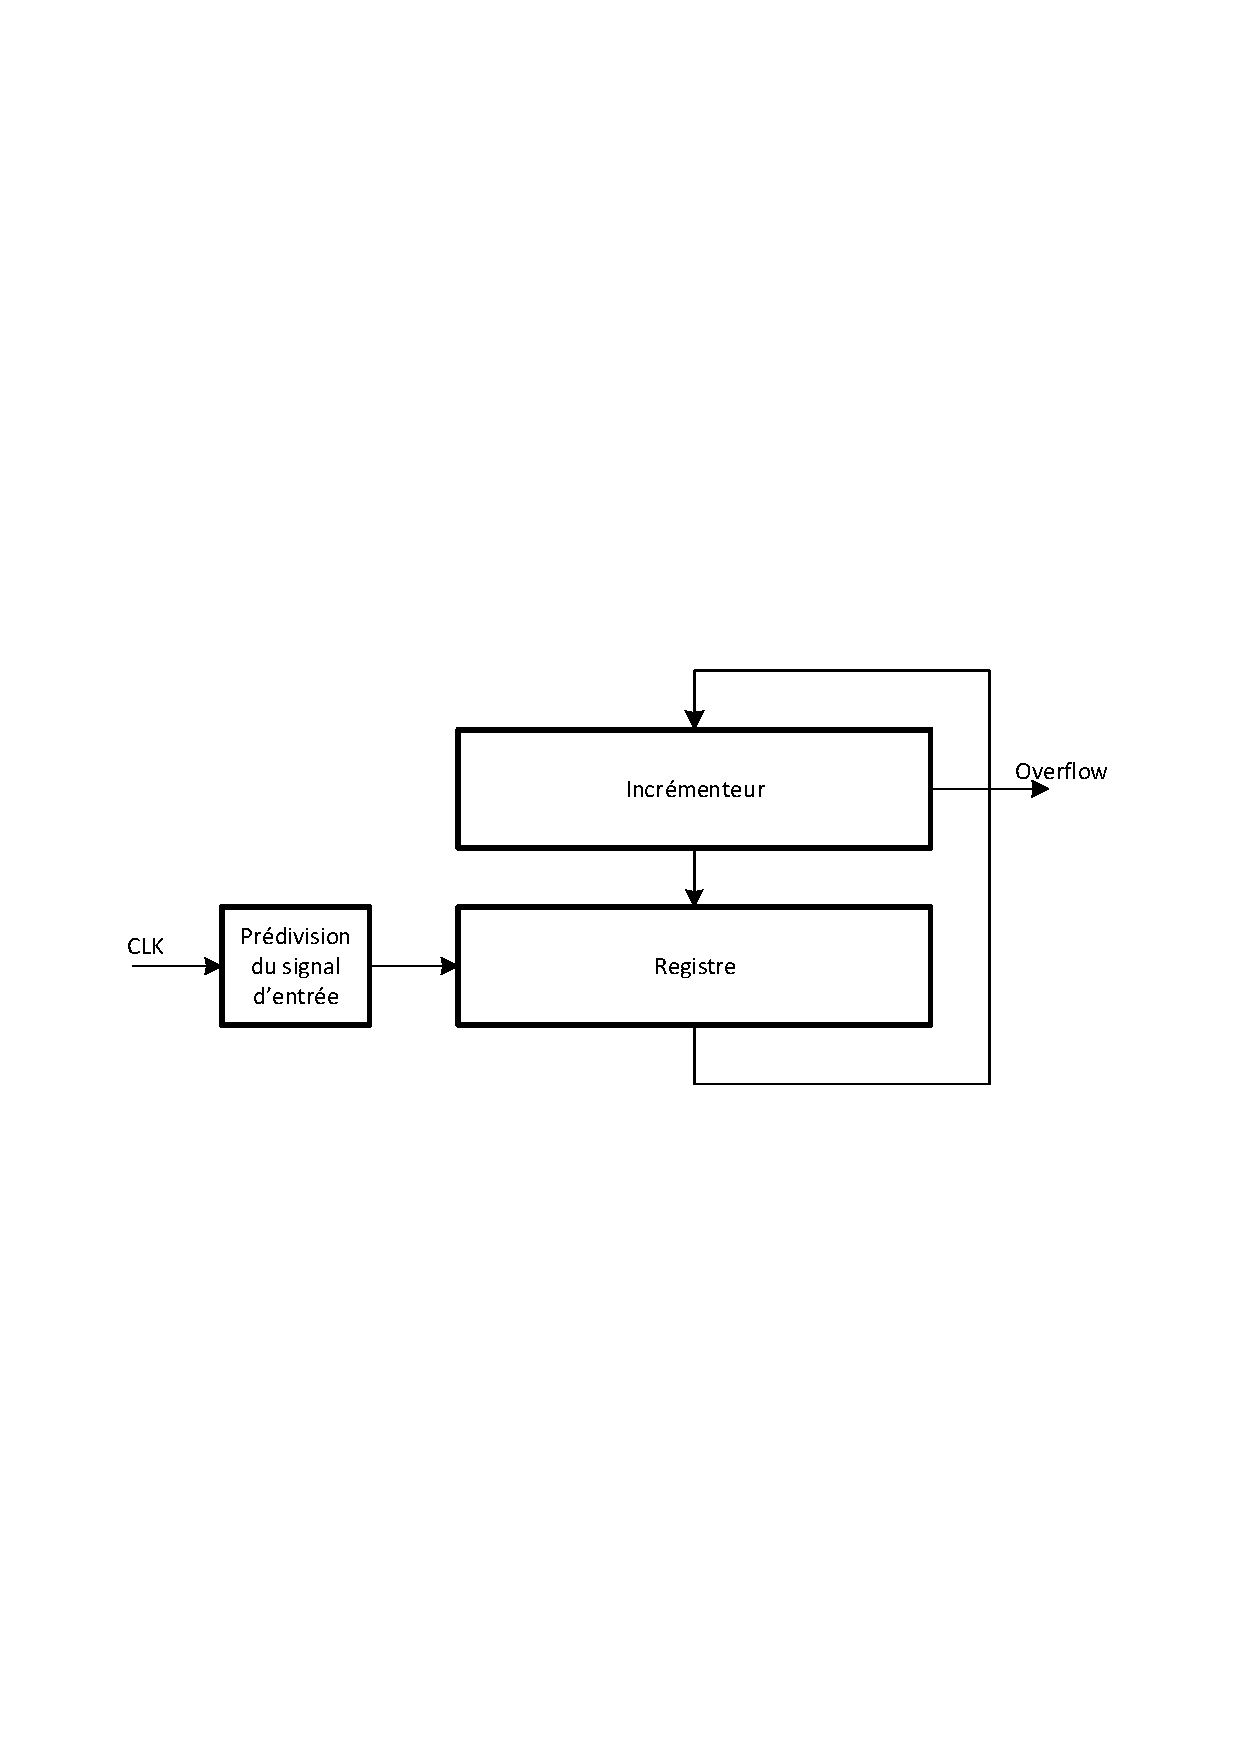
\includegraphics[angle=0, width=14cm]{./Figures/Chap5_Timer/Timer.pdf}
  \rule{35em}{0.5pt}
  \caption[Schéma Timer]{Schéma de base d'un timer}
  \label{fig:Timer}
\end{figure}

L'incrémentation se fait au rythme d'un signal souvent appelé CLK (fig. \ref{fig:Timer}), qui est soit:
\begin{itemize}[label=\textbullet,font=\small]
\item périodique, auquel cas le circuit mesure (compte) le temps, et on parle de \textit{timer};
\item apériodique quelconque, auquel cas le circuit compte simplement les flancs de ce signal tant qu'il est actif et on parle plutôt de \textit{compteur}.
\end{itemize}

Souvent, un prédiviseur de fréquence permet de réduire la fréquence du signal CLK pour ralentir le rythme du comptage.

La figure \ref{fig:ChronoSync} montre l'évolution de la valeur du registre en fonction du temps, pour un \textit{timer} de 4 bits. La pente de la courbe dépend du rythme auquel le registre est incrémenté, donc de la fréquence du signal CLK.
Lorsque le registre atteint sa valeur maximale, égale à $2^N-1$, il repasse à 0. Durant ce passage à 0, un signal (qui est la retenue sortante du circuit incrémenteur) passe à '1' et émet éventuellement une requête d'interruption.

\begin{figure}[htb]
  \centering
  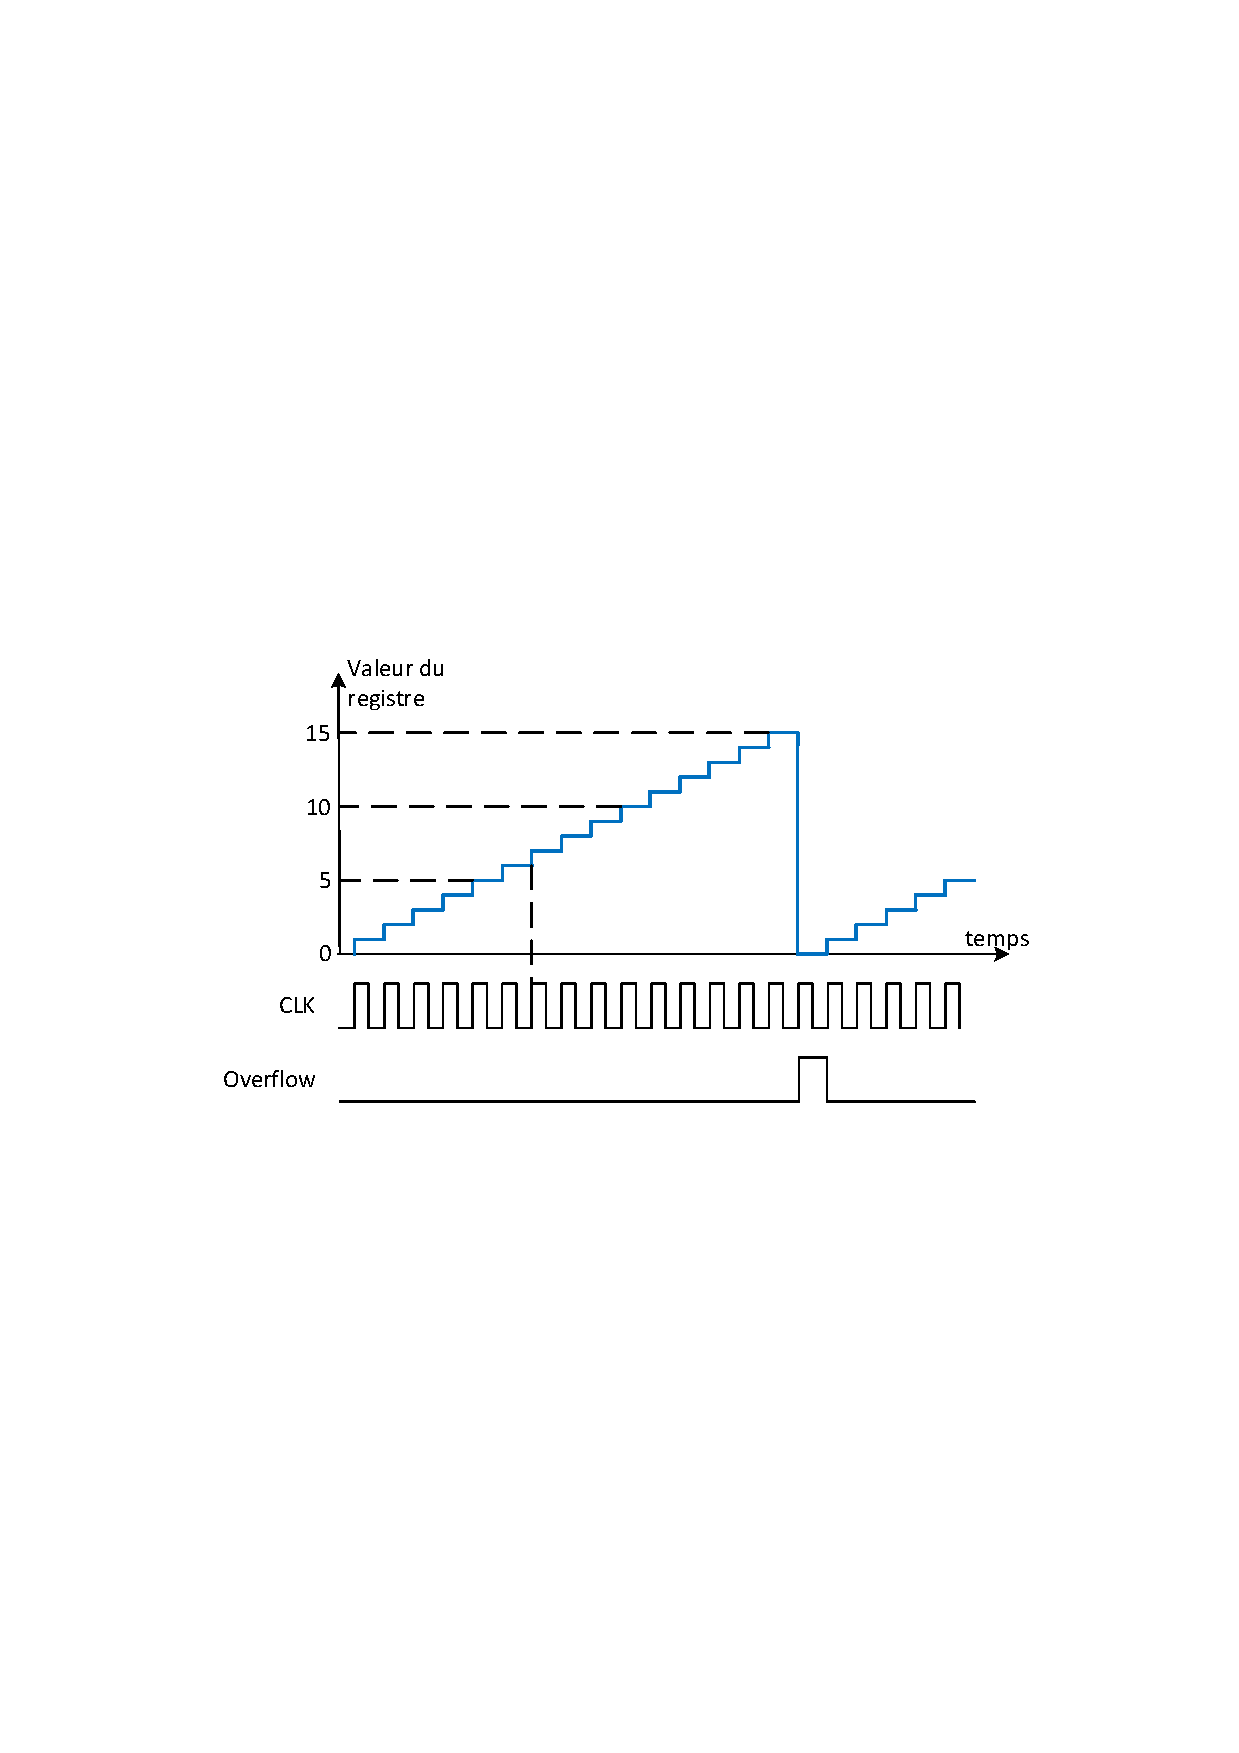
\includegraphics[angle=0, width=14cm]{./Figures/Chap5_Timer/Timer_chrono1.pdf}
  \rule{35em}{0.5pt}
  \caption[Chrono timer]{Comportement temporel du timer (N=4)}
  \label{fig:ChronoSync}
\end{figure}

Dans le cas d'un compteur, le signal CLK est apériodique. La figure \ref{fig:ChronoAsync} montre l'évolution de la valeur du registre en fonction du temps, pour un \textit{compteur} de 4 bits. De même, la retenue sortante du circuit incrémenteur émet éventuellement une requête d'interruption lors du passage par 0 de la valeur du registre.

\begin{figure}[htb]
  \centering
  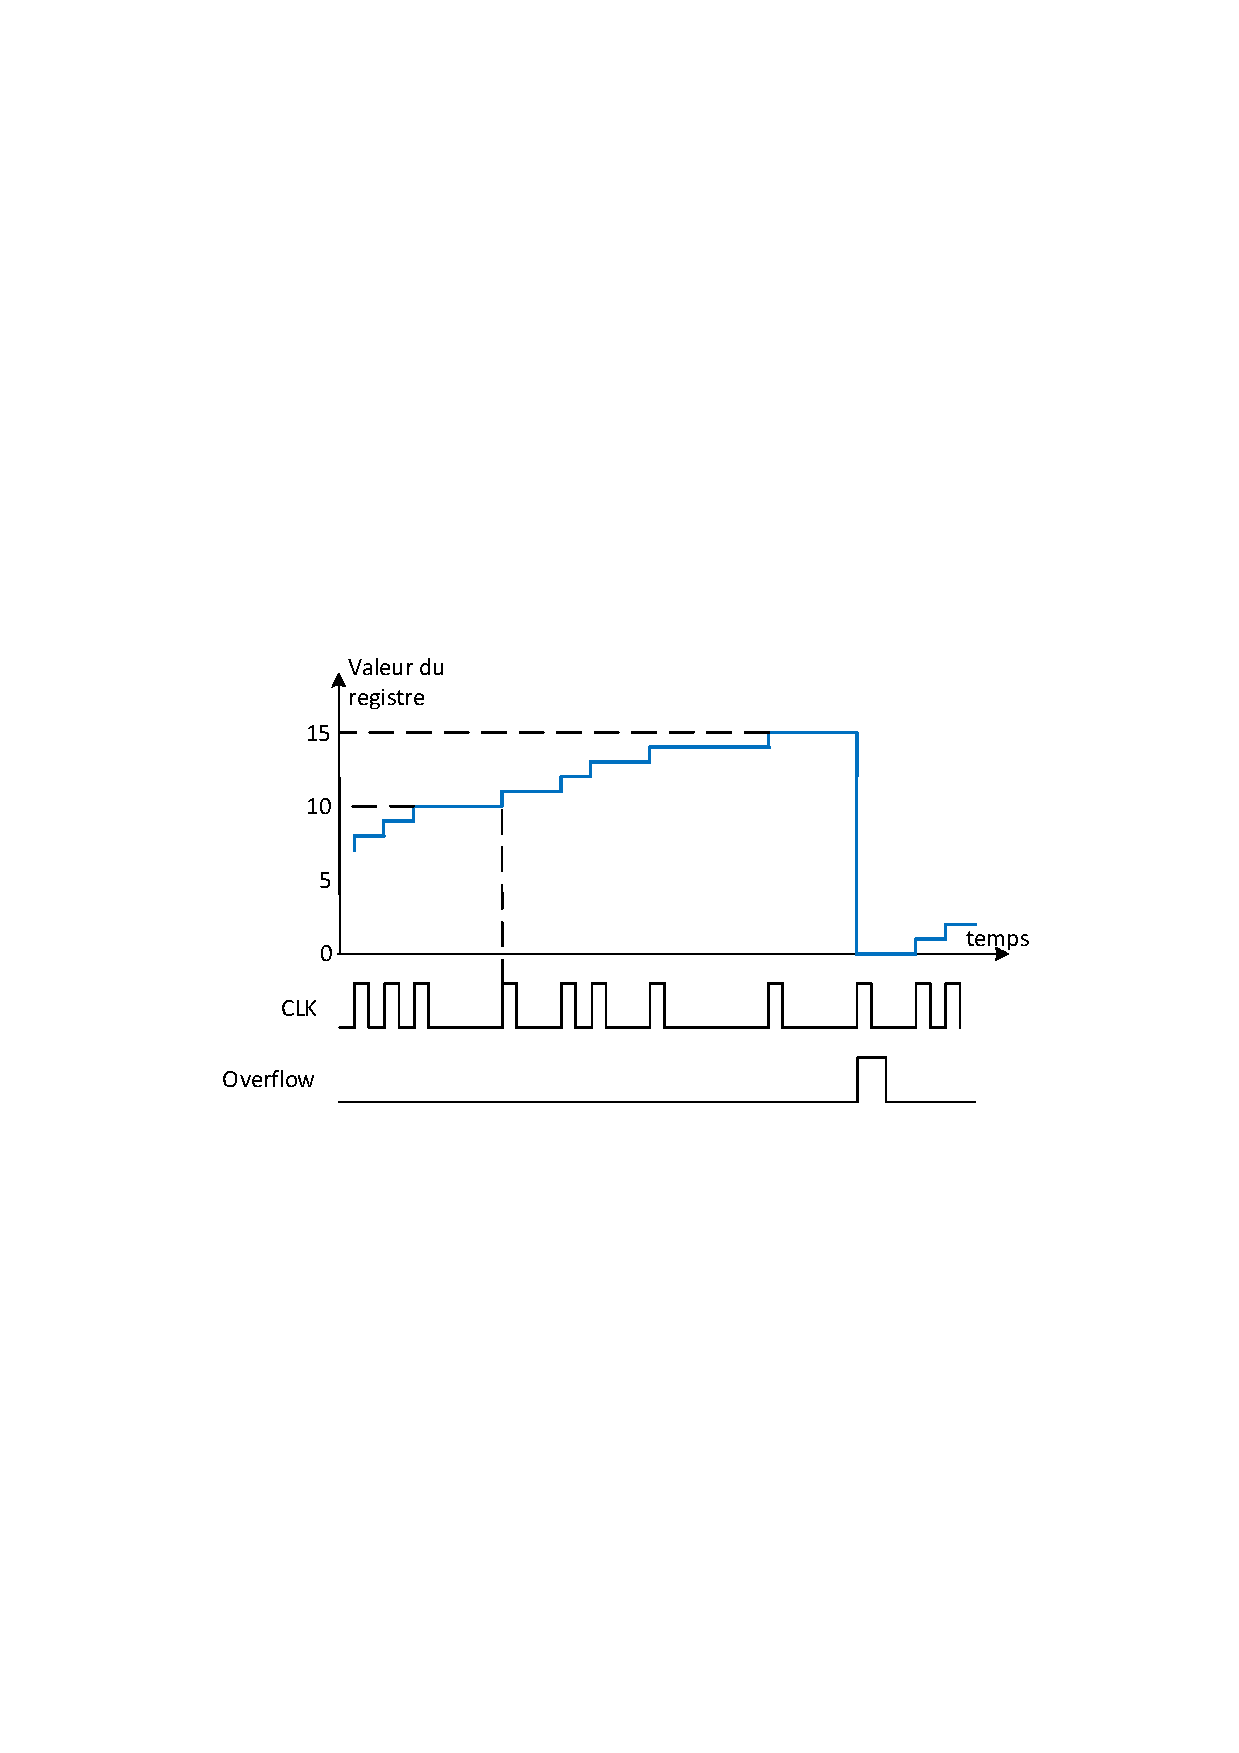
\includegraphics[angle=0, width=14cm]{./Figures/Chap5_Timer/Timer_chrono2.pdf}
  \rule{35em}{0.5pt}
  \caption[Chrono compteur]{Comportement temporel d'un compteur (N=4)}
  \label{fig:ChronoAsync}
\end{figure}

Comme nous le verrons dans la suite, certains timers utilisent un décrémenteur au lieu d'un incrémenteur, voire les deux.
Finalement, on peut rencontrer différents types de timers dans un même microcontrôleur, chacun étant adapté à un besoin spécifique.

\section{Cas du MSP430}
Les microcontrôleurs de la famille MSP430 embarquent jusqu'à 5 types de timers différents:
\begin{itemize}[label=\textbullet,font=\small]
\item Real Time Clock, ou \textit{Horloge Temps Réel} (RTC) pour la création d'horloges
\item WatchDog Timer ou \textit{Chien de Garde} (WDT) pour la prévention de plantées d'origines diverses
\item 3 types de timers à usage général
\end{itemize}

\subsection{Real Time Clock}
Après initialisation, le RTC maintient à jour les informations horaires les plus courantes:
\begin{itemize}[label=\textbullet,font=\small]
\item année
\item numéro du mois dans l'année
\item jour du mois
\item jour de la semaine
\item heure
\item minute
\item seconde
\end{itemize}

Ce type de timer nécessite une horloge dont la fréquence est 1Hz, dérivée d'une horloge standard à 32768Hz. Cette dernière fréquence fut introduite aux débuts de la montre à quartz car il est aisé de réaliser des quartz à cette fréquence. On obtient l'horloge à 1Hz par une simple division de 32768 par $2^{15}$.

\subsection{WatchDog Timer}
La "plantée" d'un programme est la plupart du temps due à un défaut dans le programme ou à un concours de circonstances qui fait que le programme est bloqué dans un boucle sans fin. Le cas le plus courant est l'attente d'un évènement qui n'arrive pas et qui n'arrivera jamais.
Le microcontrôleur ne réagit plus. Le seul moyen est de le \textit{resetter}.
Un timer \textit{chien de garde} resette donc le CPU, donc le programme, si celui-ci ne l'a pas remis à 0 avant.
Lors du développement, on désactive généralement le chien de garde. Dans le MSP430, ceci est effectué au moyen de l'instruction :

\lstset{style=customc}
\begin{lstlisting}
WDTCTL = WDTPW +WDTHOLD;
\end{lstlisting}
En opération, cette instruction est mise en commentaire. Le chien de garde est alors actif, et il est nécessaire d'ajouter des instructions dans les boucles d'attente et à des endroits bien choisis du programme pour le remettre à 0 avant qu'il ne force le programme à redémarrer.

\section{Timer à usage général : le timer A}
Dans le MSP430, le timer à usage général est un périphérique complexe auquel le CPU peut soutraiter des fonctionnalités sophistiquées. En plus des fonctionnalités usuelles, on trouve:
\begin{itemize}[label=\textbullet,font=\small]
\item capture de l'état du registre de comptage lors d'un évènement
\item requêtes d'interruption dès que le registre de comptage \textit{est égal à} une constante donnée (comparaison)
\item génération de signaux PWM sur une patte externe, sans aucune aide du CPU autre que l'initialisation
\end{itemize}
Toutes ces fonctionnalités sont contrôlées par le logiciel, en positionnant des champs logiques dans des registres de contrôle. Un champ logique est un groupe de variables logiques dans un registre.

Dans une version de MSP430 donnée, plusieurs Timers A peuvent coexister.

La figure \ref{fig:TimerAsimplifie} est un schéma très simplifié du timer A, illustrant ses 3 principaux sous-blocs. A la partie supérieure, on retrouve le bloc de comptage et son registre appelé TAxR (x est le numéro du timer; x=0 ou 1 s'il y a deux timers de type A dans le microcontrôleur). TAIFG est le signal d'overflow du compteur. En dessous, le bloc dit de "capture/comparaison" permet de capturer l'état du registre TAxR lors d'un évènement ou de comparer la valeur de TAxR avec une constante contenue dans un registre appelé TAxCCRy. Le bloc de "capture/comparaison" contient un sous-bloc, noté "Output module", qui est chargé de générer un signal PWM à partir du contenu du registre TAxR et de la constante contenue dans le registre TAxCCRy.
Comme on le voit sur la figure \ref{fig:TimerAsimplifie}, Chaque sous-bloc offre de la fonctionnalité utile.

\begin{figure}[htb]
  \centering
  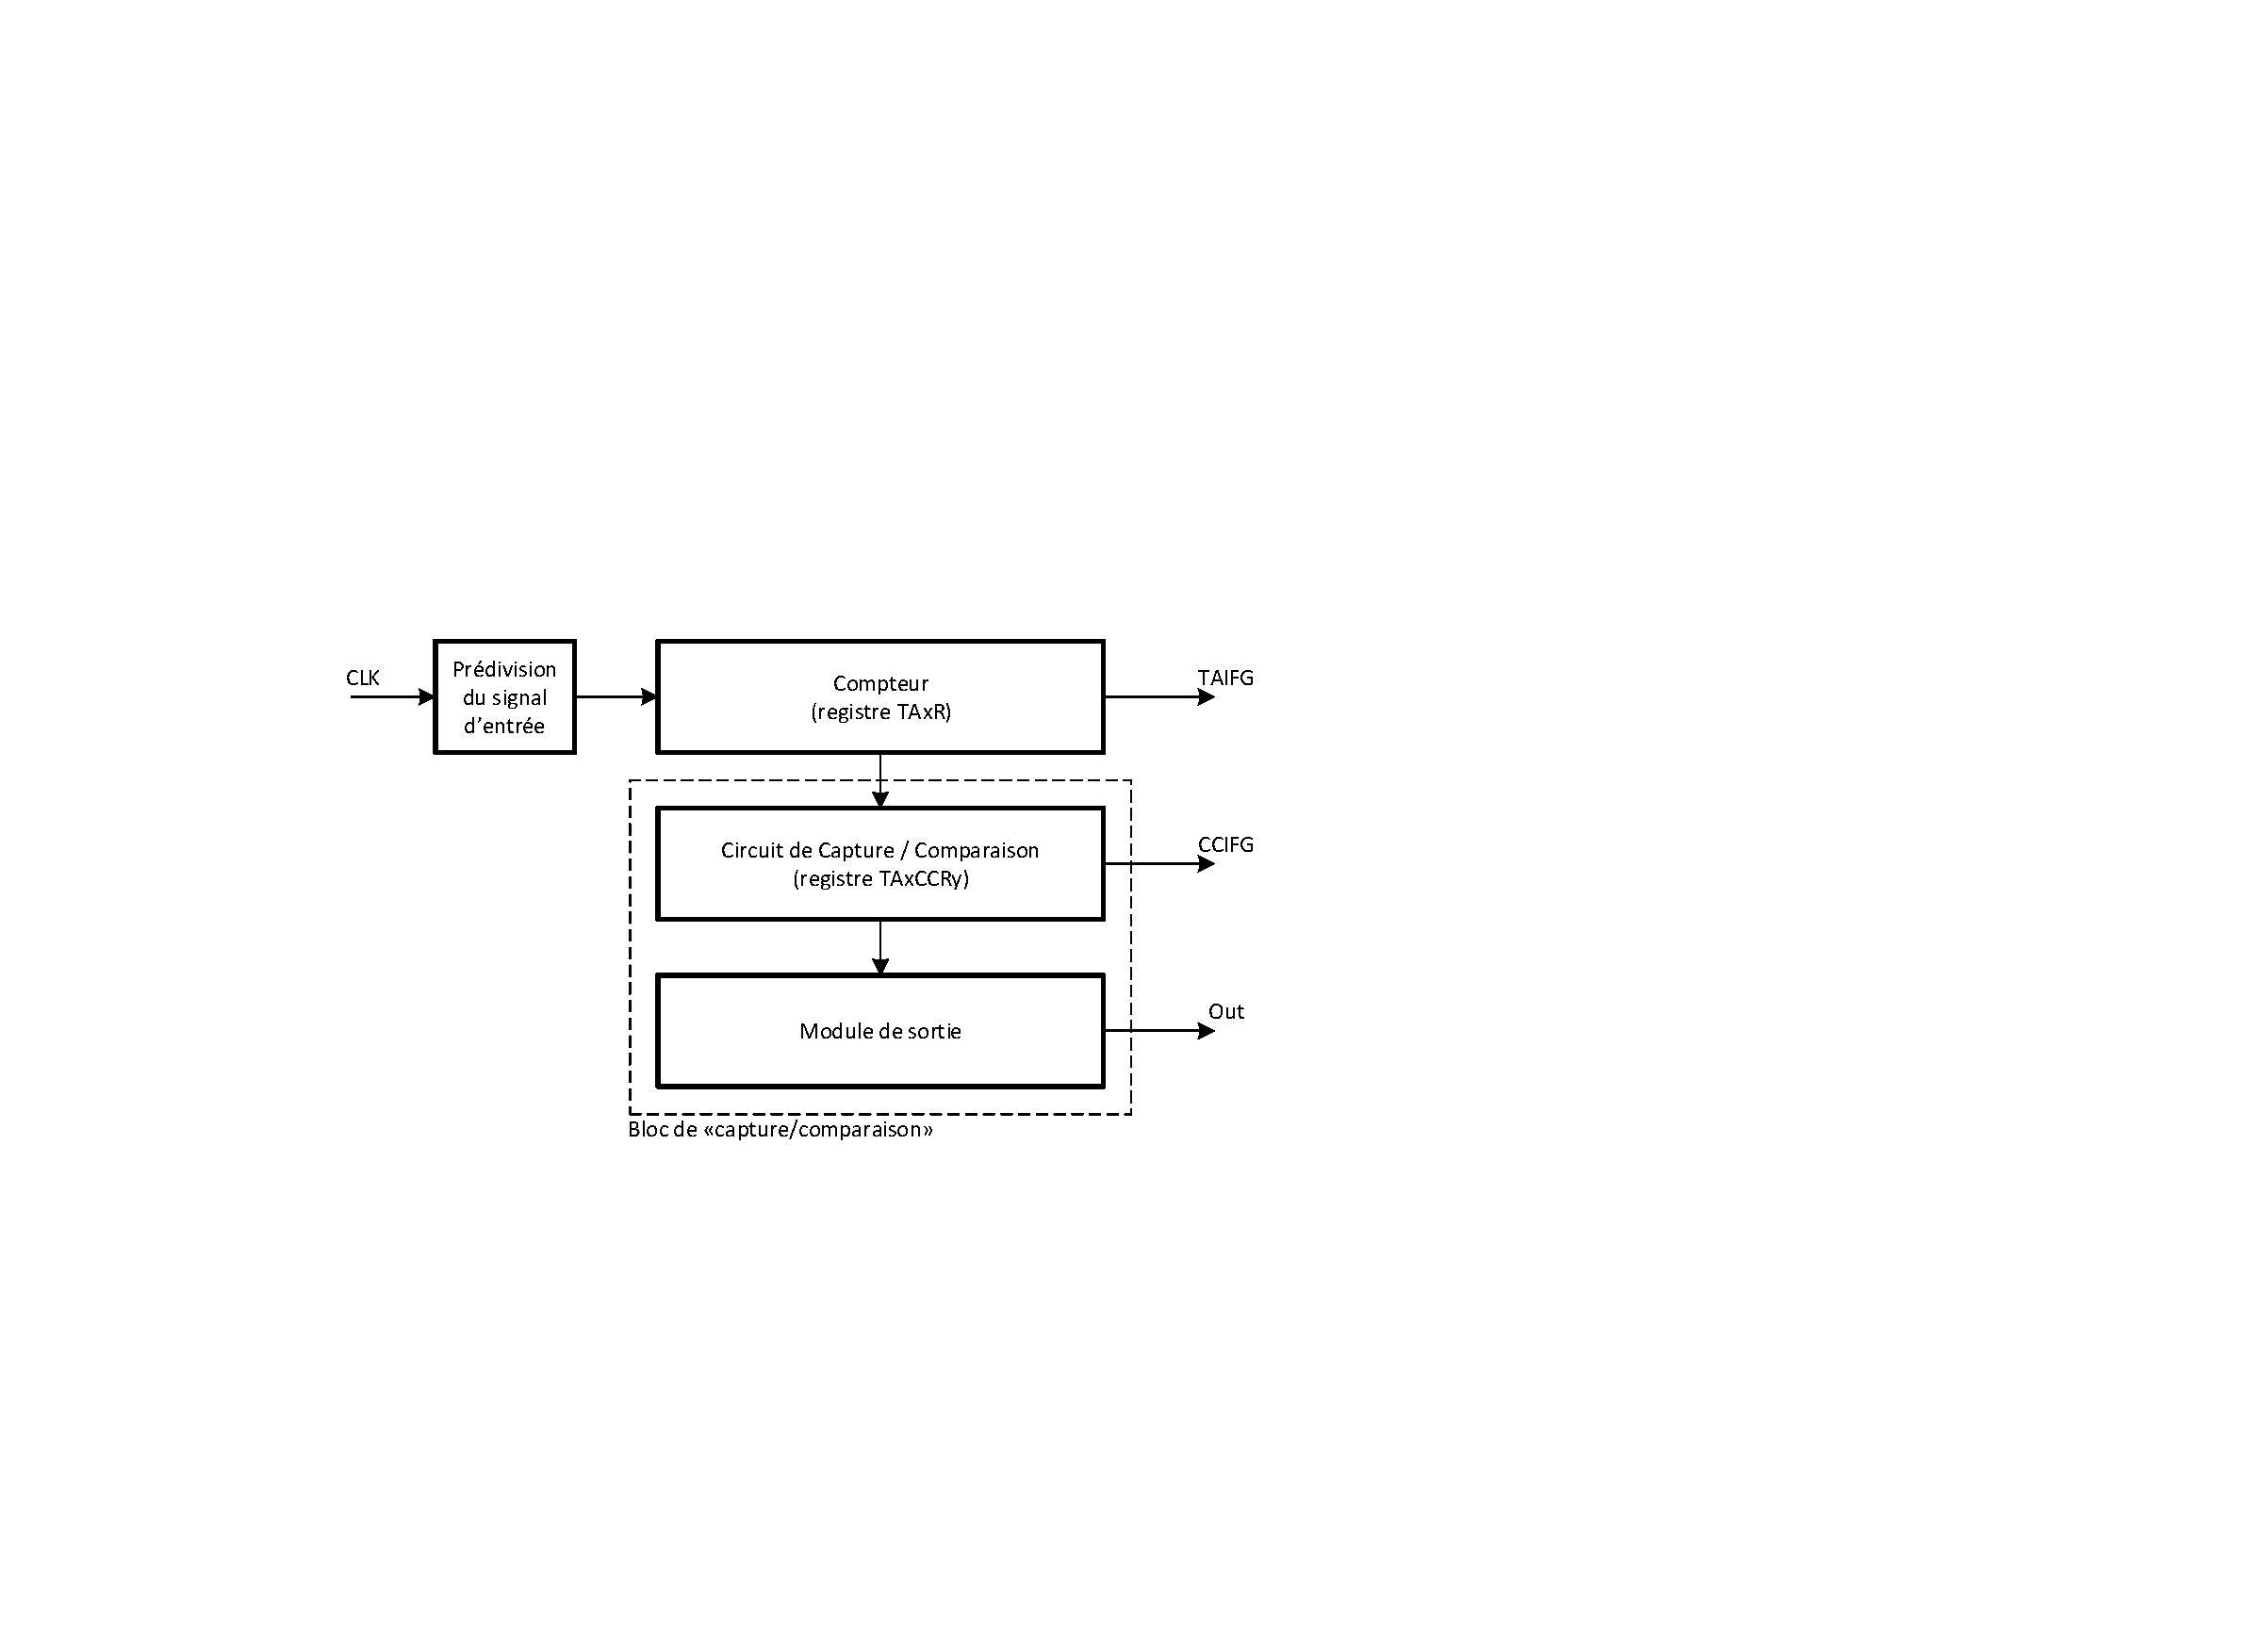
\includegraphics[angle=0, width=14cm]{./Figures/Chap5_Timer/Timer_blocs_1.pdf}
  \rule{35em}{0.5pt}
  \caption[TimerA simplifie]{Schéma simplifié du timer A}
  \label{fig:TimerAsimplifie}
\end{figure}


\subsection{Bloc de comptage}
La figure \ref{fig:TimerTAR} illustre en détail le bloc de comptage. On y voit les différents éléments et leurs champs de contrôle, tous inclus dans un registre de contrôle appelé TAxCTL, que nous verrons plus loin.

\begin{figure}[H]
  \centering
  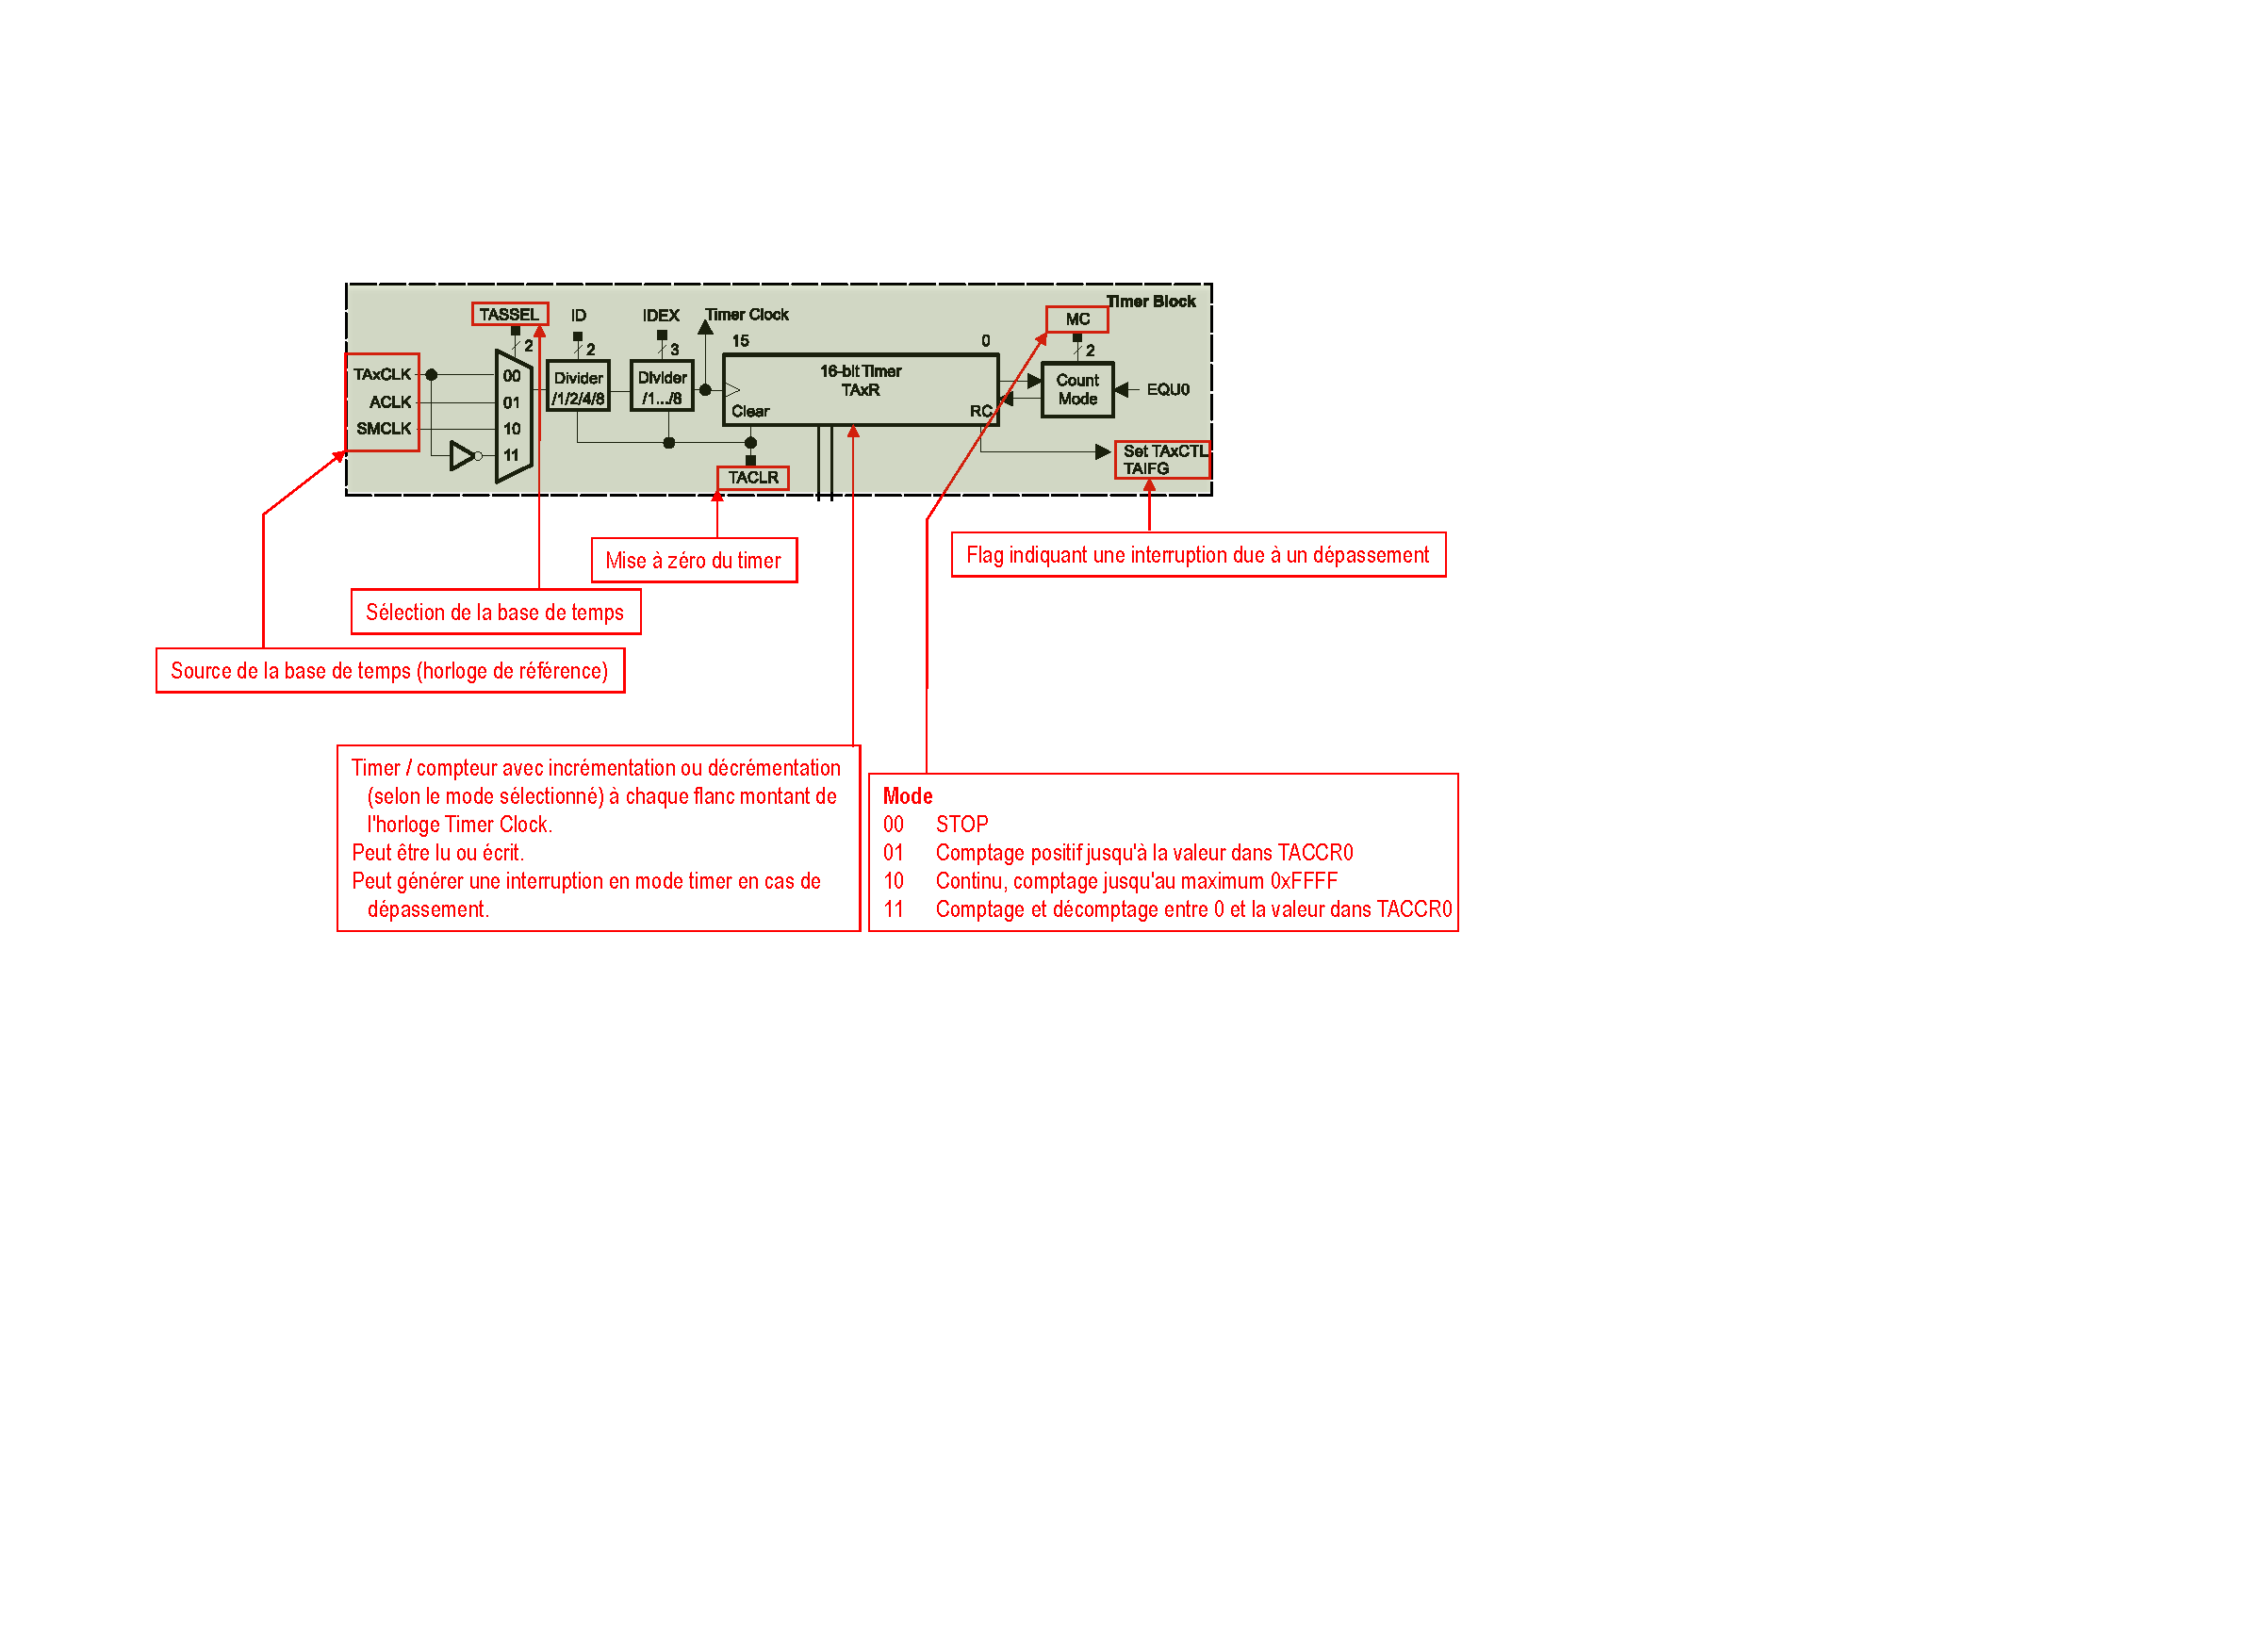
\includegraphics[angle=0, width=16cm]{./Figures/Chap5_Timer/Timer_Detail_1.pdf}
  \rule{35em}{0.5pt}
  \caption[TimerTAR]{Schéma de détail du bloc de comptage}
  \label{fig:TimerTAR}
\end{figure}

Le registre de comptage TAxR a 3 modes de comptage possibles. Le mode est déterminé par la valeur du champ MCx dans le registre de contrôle TACTLx:
\begin{itemize}[label=\textbullet,font=\small]
\item Mode 1 (MCx = 01): Comptage jusqu'à la valeur contenue dans le registre TAxCCR0, localisé dans un sous-bloc de capture/comparaison, puis retour à 0;
\item Mode 2 (MCx = 10): Comptage jusqu'à 0xFFFF, puis retour à 0;
\item Mode 3 (MCx = 11): Comptage jusqu'à la valeur contenue dans le registre TAxCCR0, puis décomptage jusqu'à 0.
\end{itemize}

Les figures \ref{fig:TimerAmode1}, \ref{fig:TimerAmode2} et \ref{fig:TimerAmode3a} montrent les chronogrammes associés à chaque mode.
\begin{figure}[H]
  \centering
  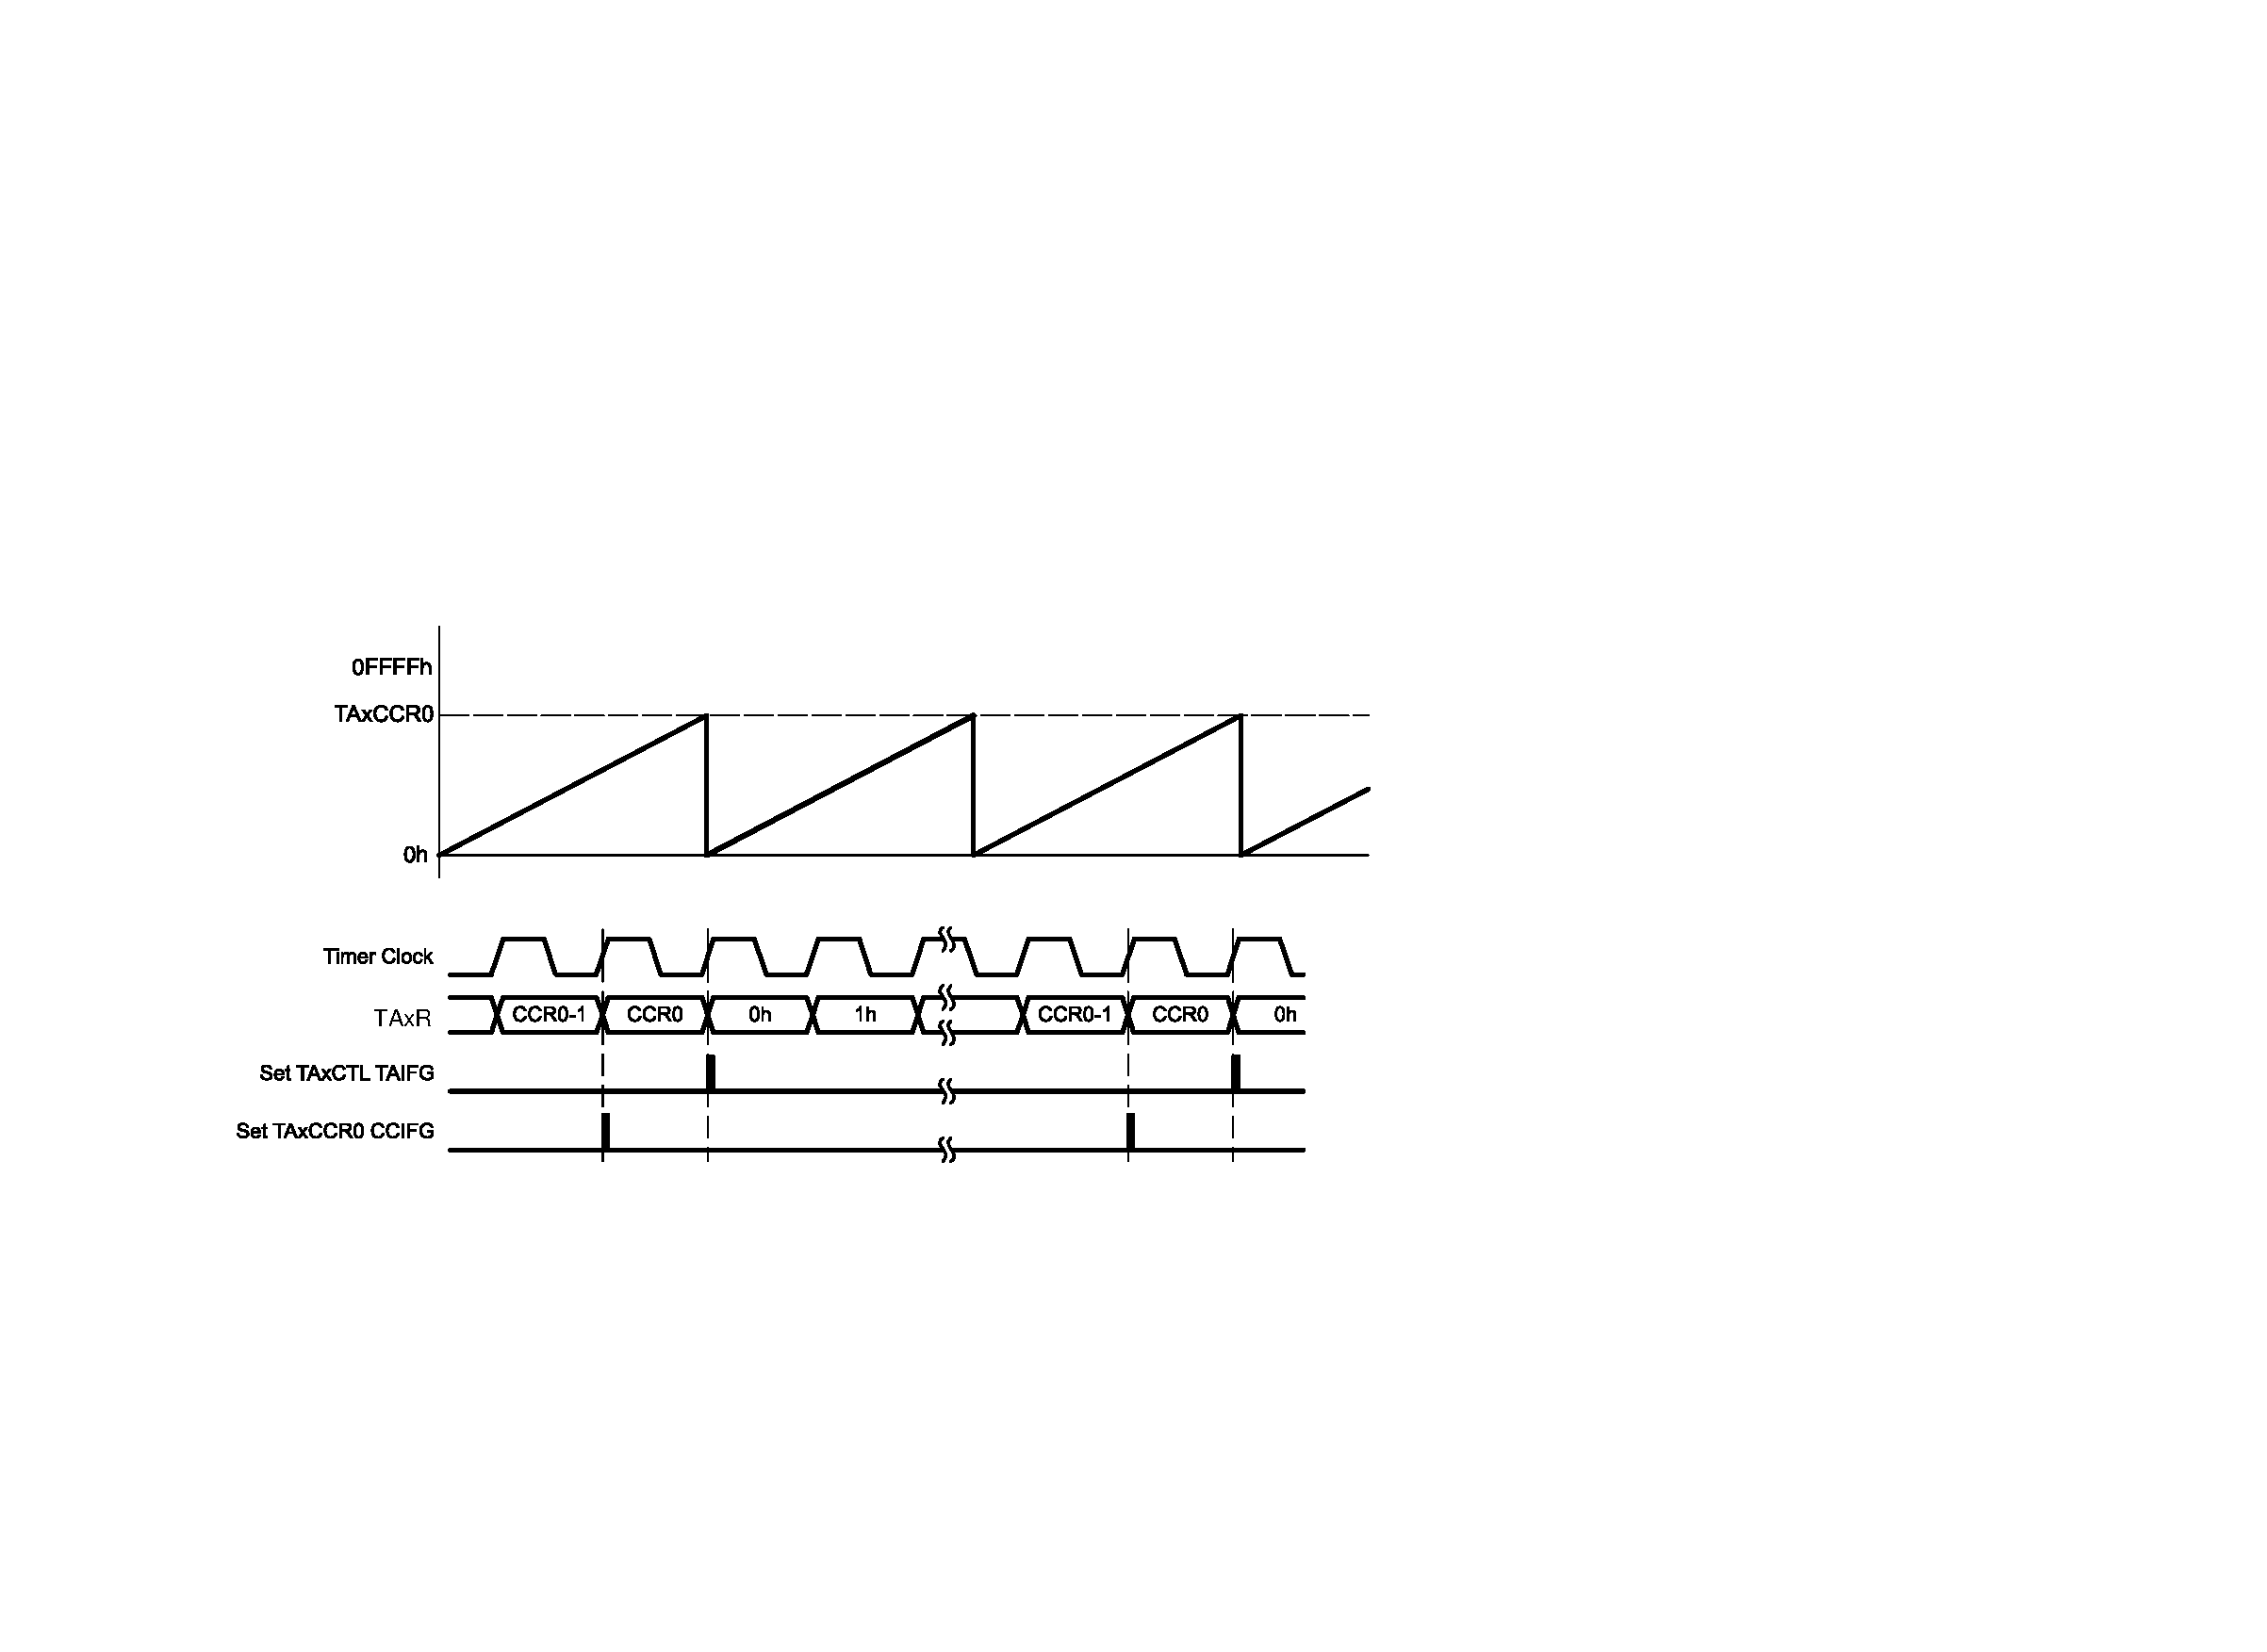
\includegraphics[angle=0, width=14cm]{./Figures/Chap5_Timer/Timer_Mode_1.pdf}
  \rule{35em}{0.5pt}
  \caption[TimerA Mode 1]{Comptage en mode 1 (MCx = 01)}
  \label{fig:TimerAmode1}
\end{figure}

\begin{figure}[H]
  \centering
  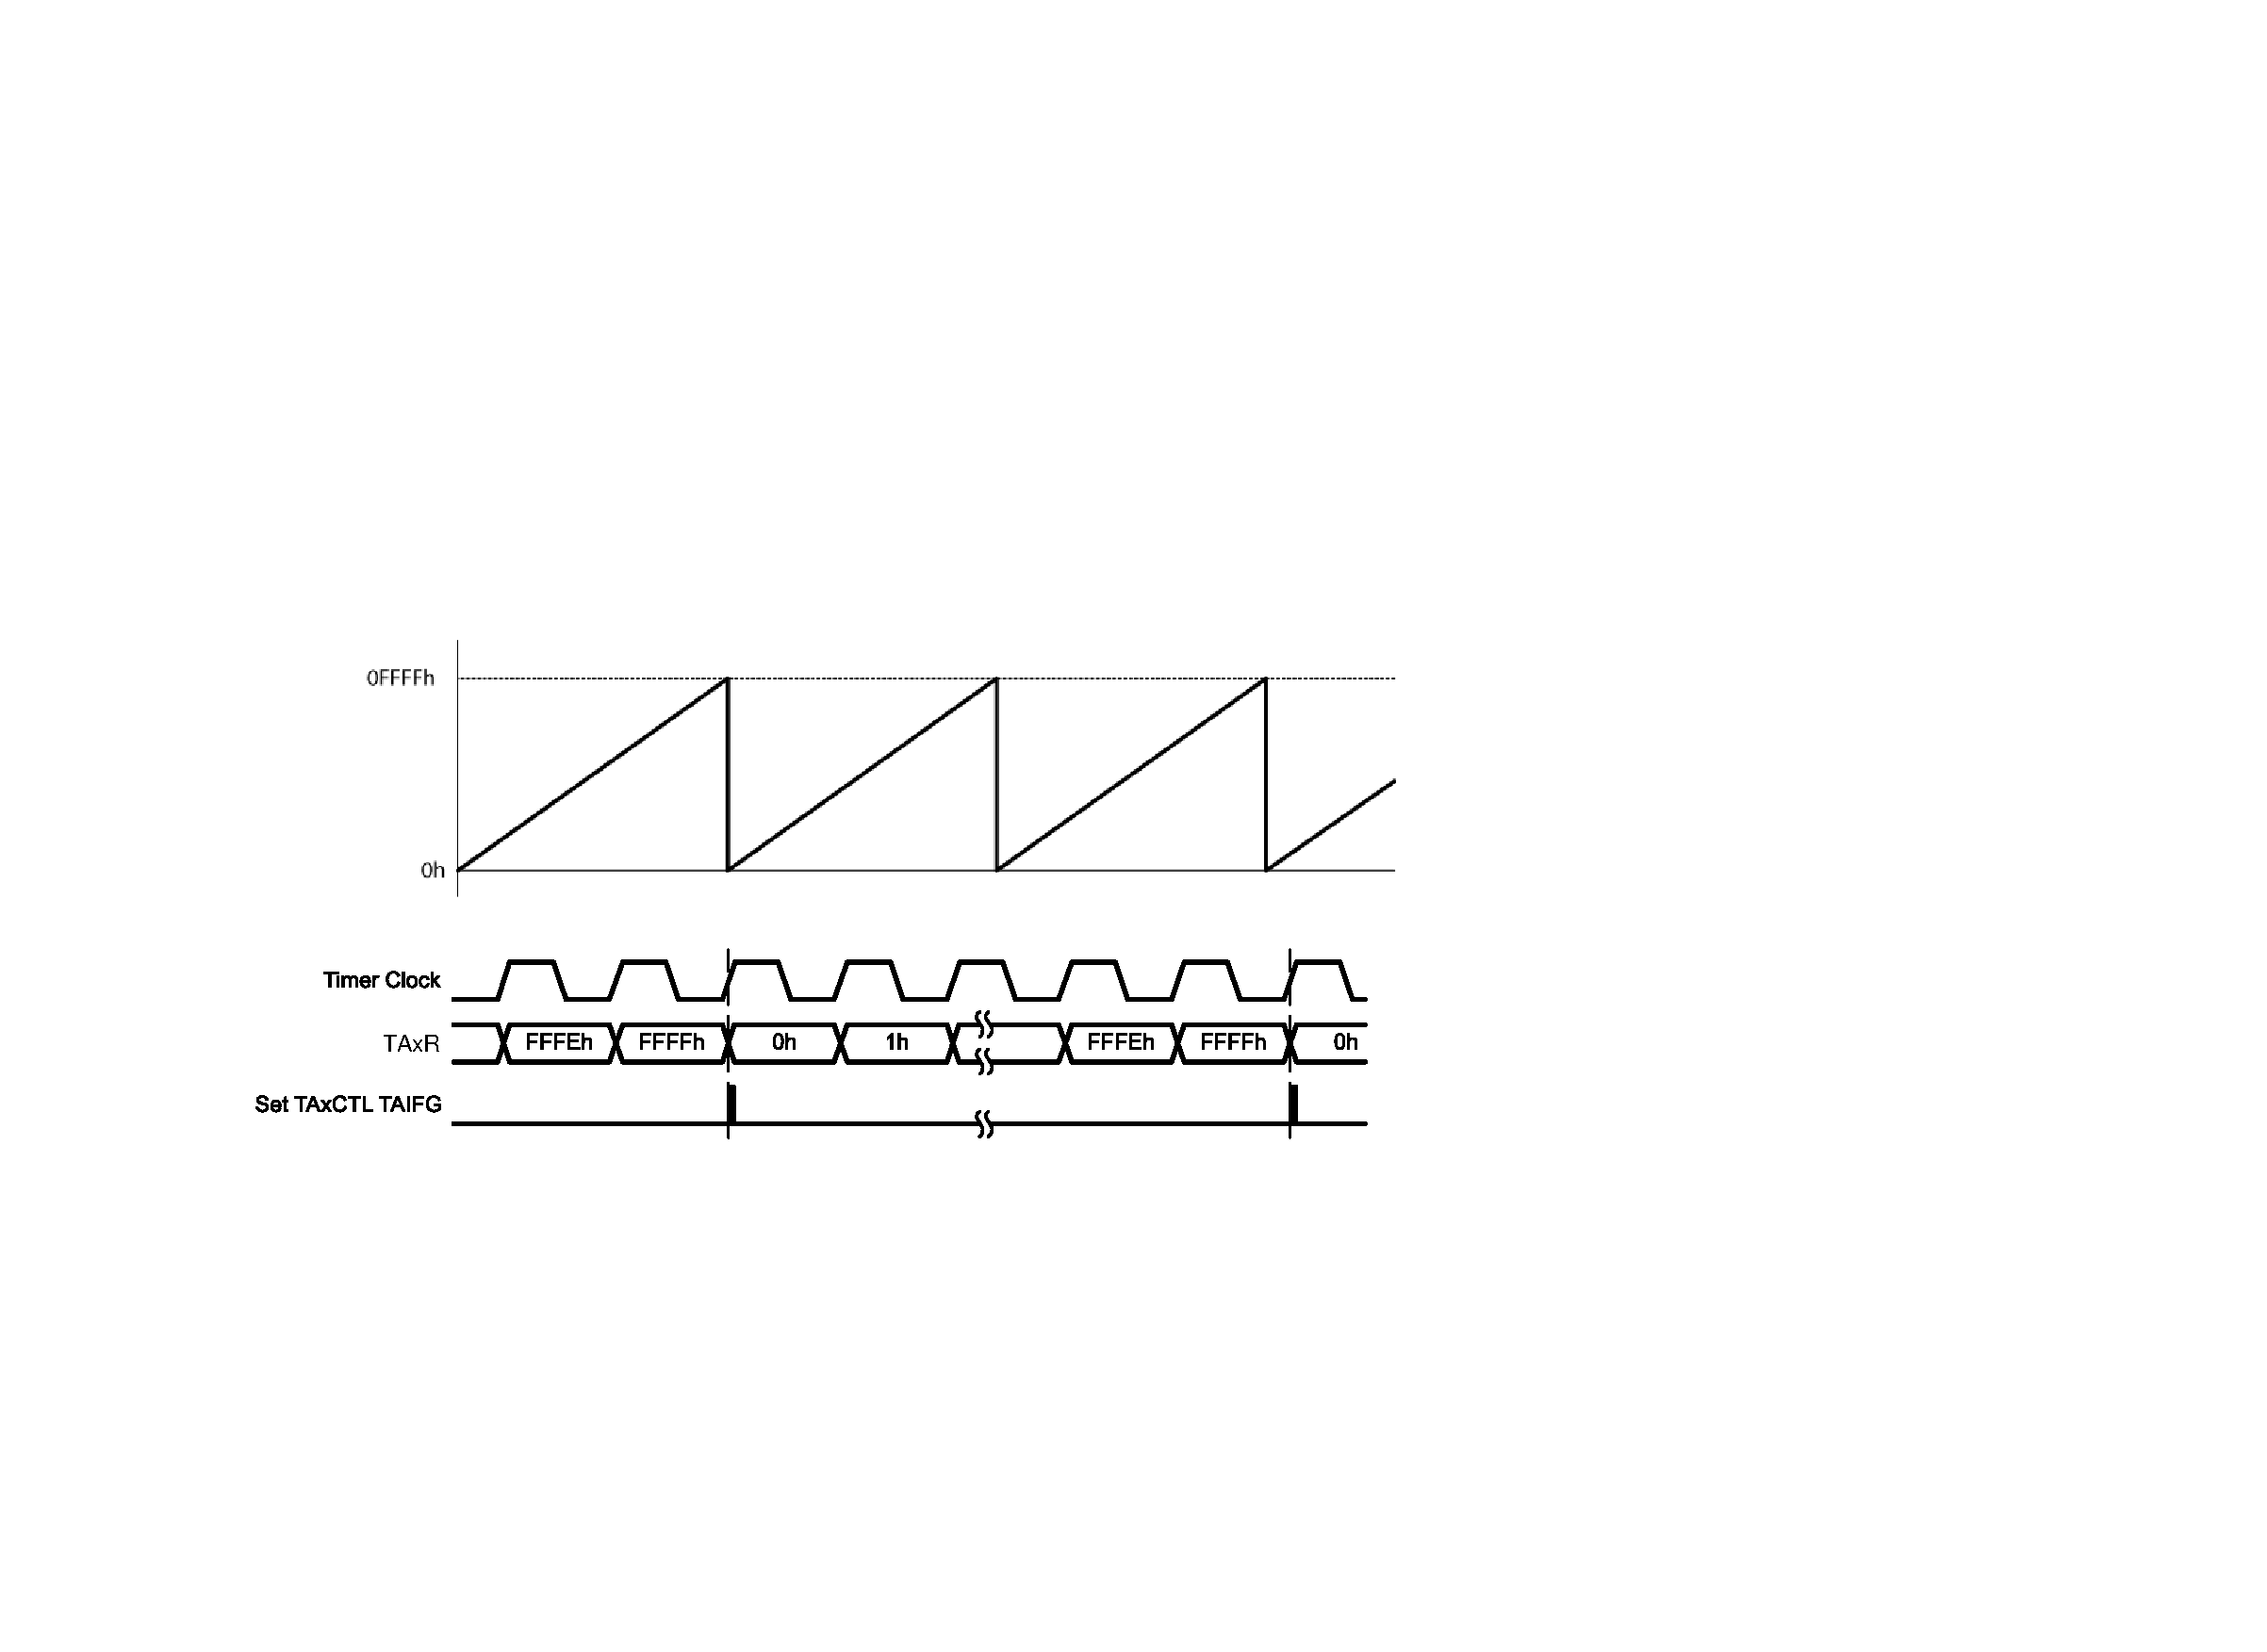
\includegraphics[angle=0, width=14cm]{./Figures/Chap5_Timer/Timer_Mode_2.pdf}
  \rule{35em}{0.5pt}
  \caption[TimerA Mode 2]{Comptage en mode 2 (MCx = 10)}
  \label{fig:TimerAmode2}
\end{figure}

\begin{figure}[H]
  \centering
  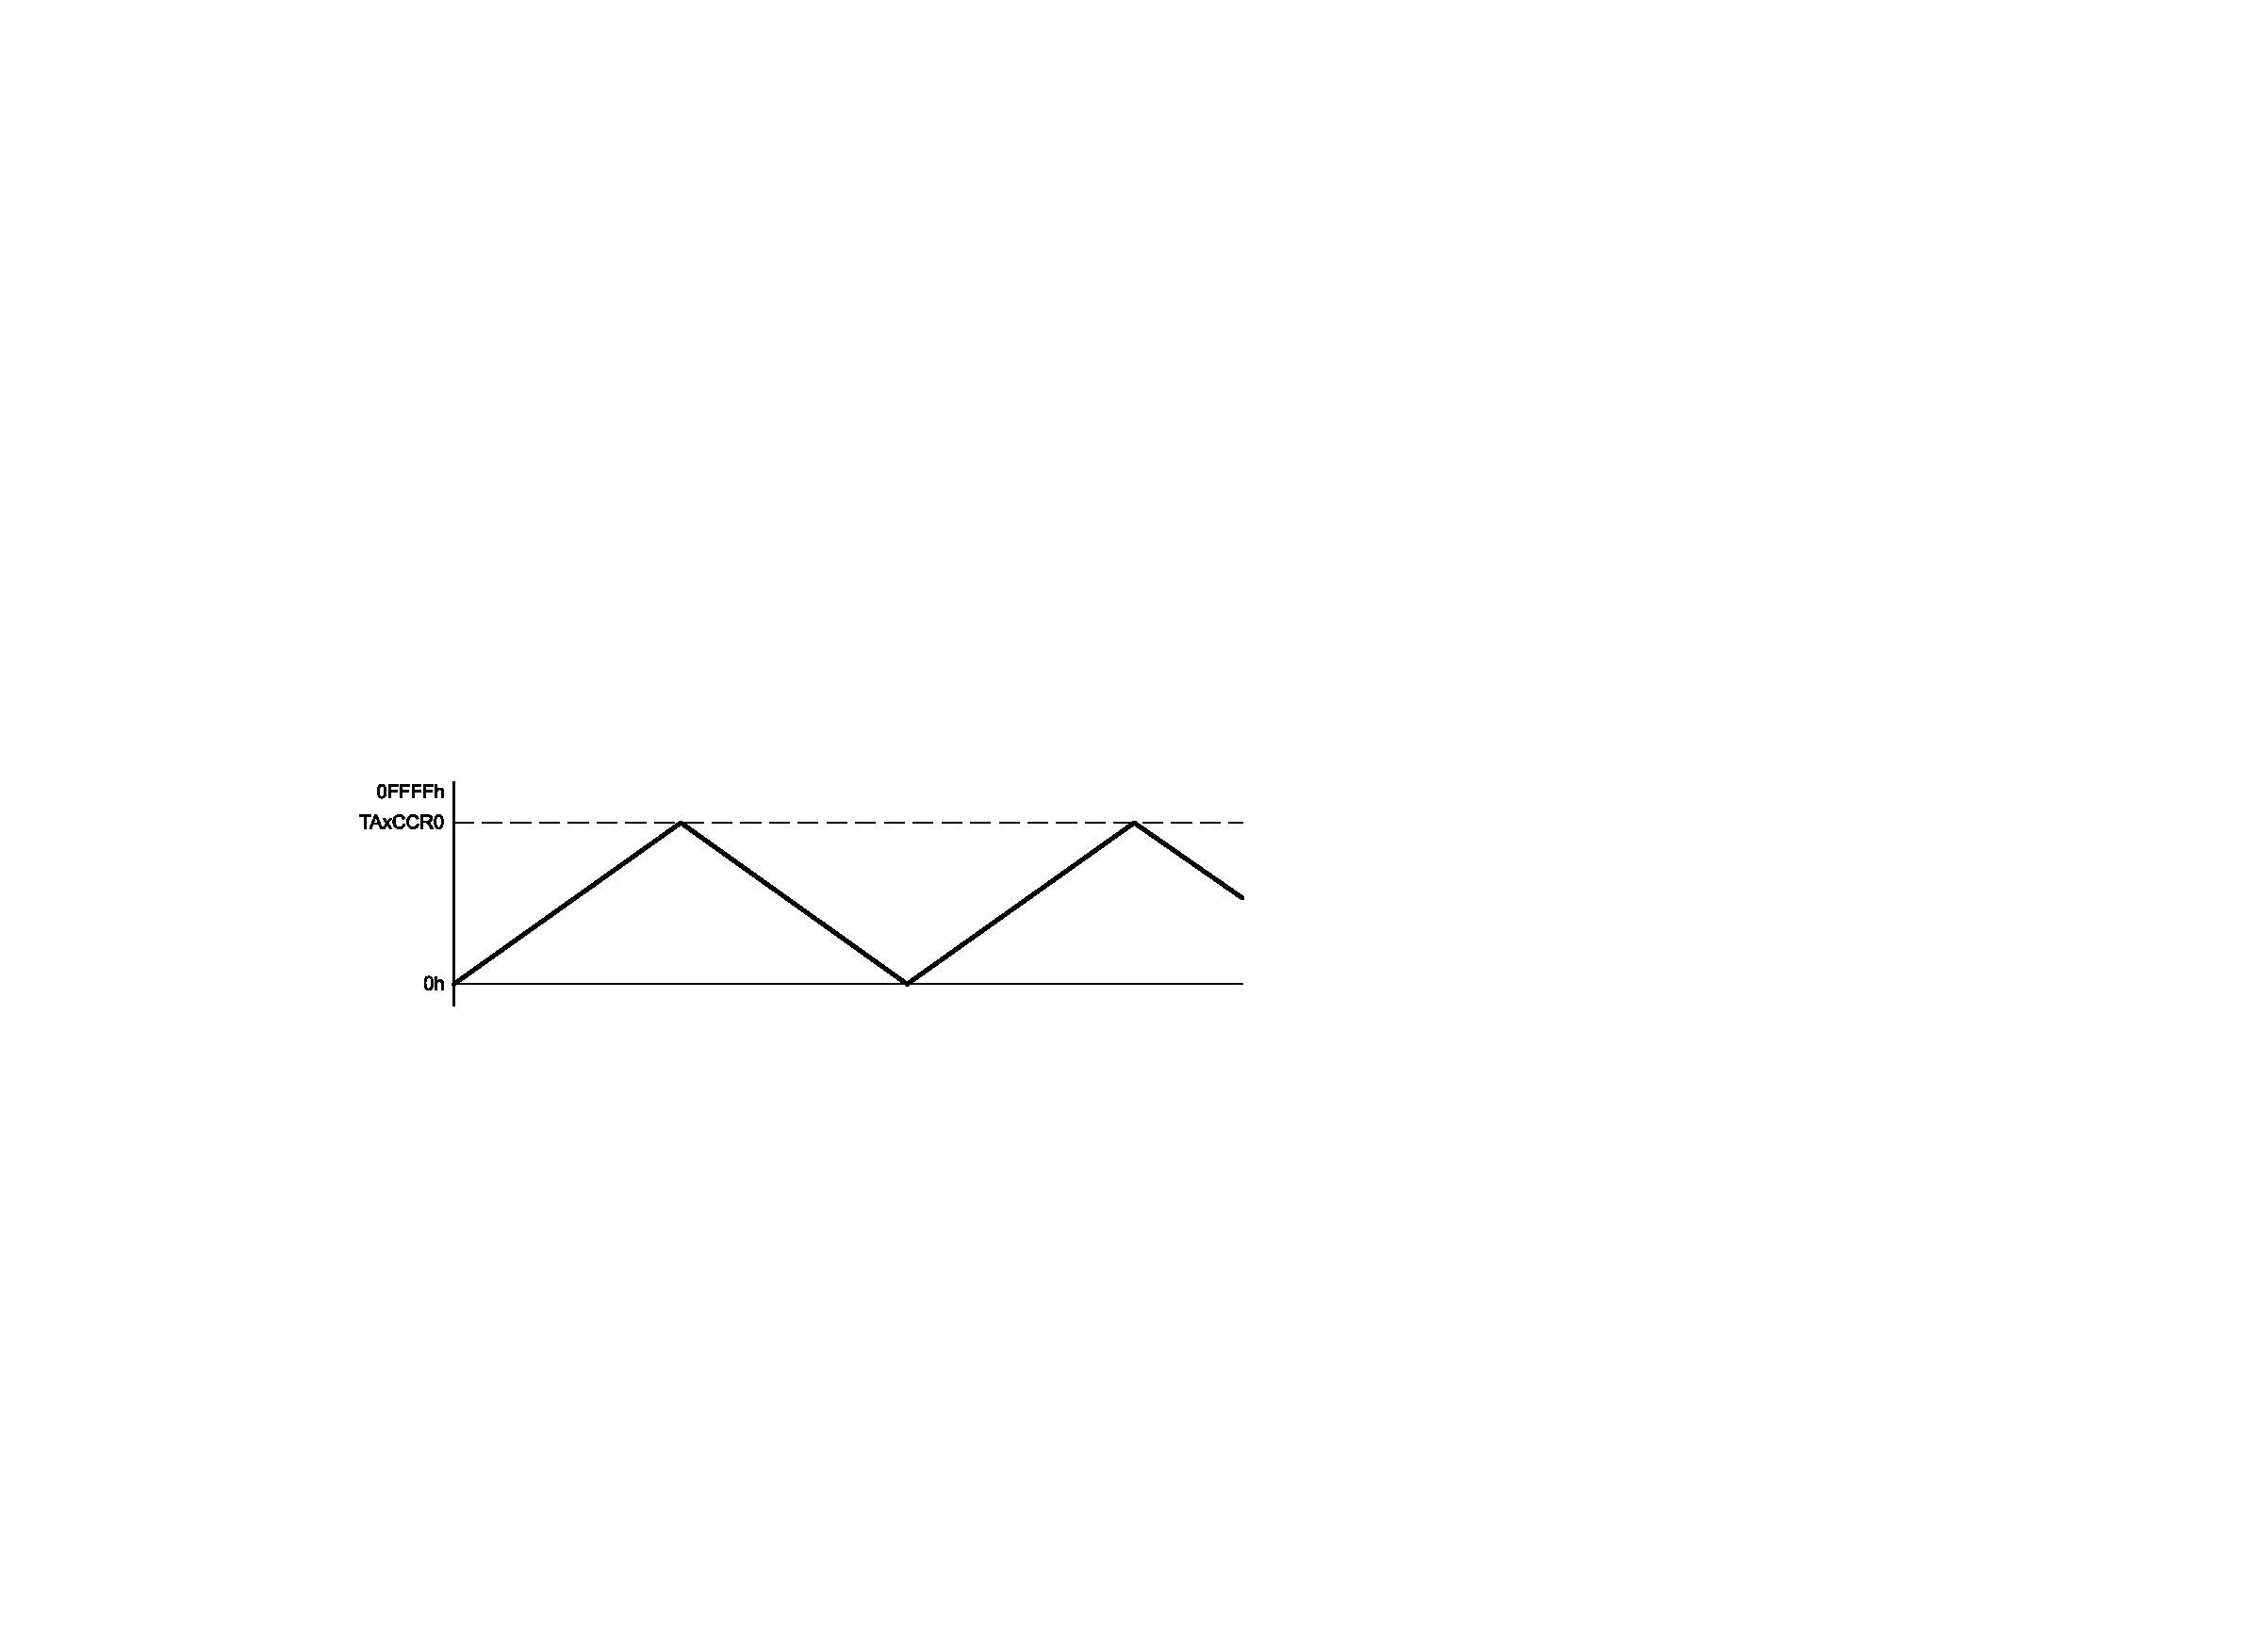
\includegraphics[angle=0, width=12cm]{./Figures/Chap5_Timer/Timer_Mode_3a.pdf}
  \rule{35em}{0.5pt}
  \caption[TimerA Mode 3]{Comptage en mode 3 (MCx = 11)}
  \label{fig:TimerAmode3a}
\end{figure}

Dans le cas du mode 3, la figure  \ref{fig:TimerAmode3b} précise le comportement des signaux TAIFG et du signal de sortie CCIFG du bloc de capture/comparaison n°0 (celui qui contient le registre TAxCCR0).
\begin{figure} [H]
  \centering
  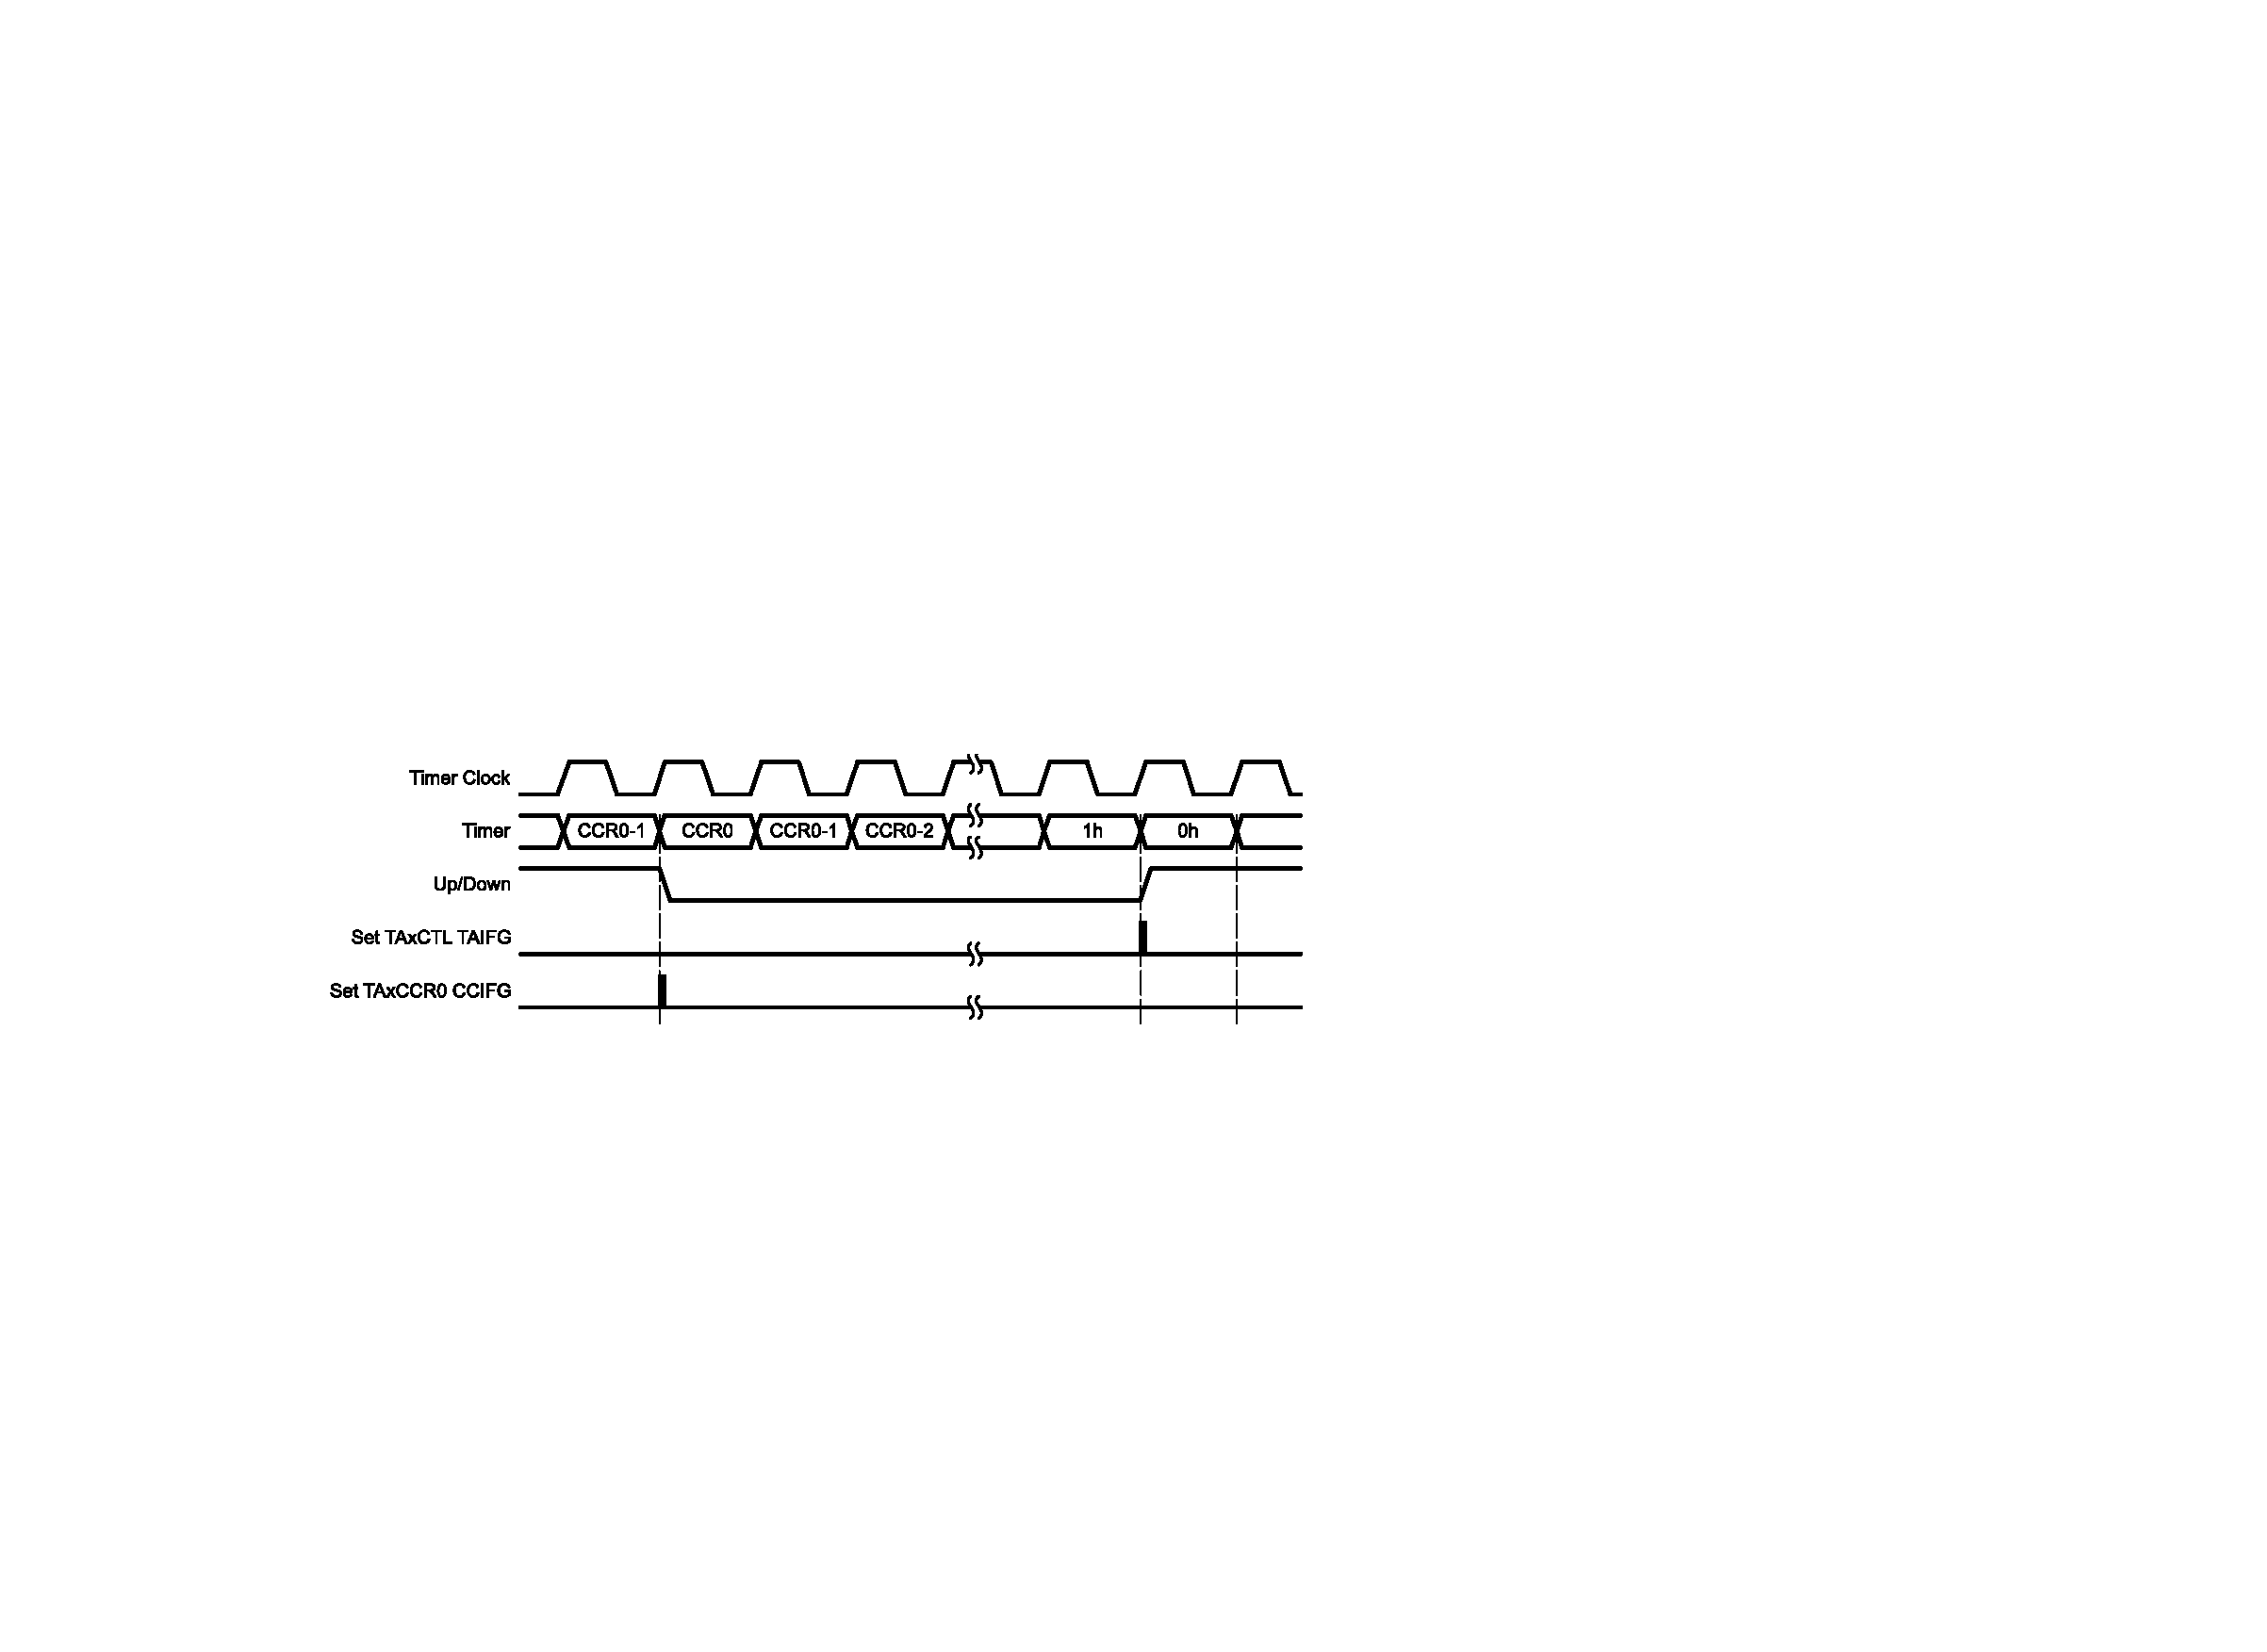
\includegraphics[angle=0, width=12cm]{./Figures/Chap5_Timer/Timer_Mode_3b.pdf}
  \rule{35em}{0.5pt}
  \caption[TimerA Mode 3]{Comptage en mode 3: détail des signaux CCIFG et TAIFG)}
  \label{fig:TimerAmode3b}
\end{figure}

Grâce à cette variété des modes de comptage, le timer A va être capable de générer un grand nombre de signaux différents.

\subsection{Contrôle du bloc de comptage}
TAxR : Timer A Register (n° x) ou registre de comptage du timer n° x. Sa valeur évolue entre 0 et 0xFFFF ou le contenu de TAxCCR0.

TAxCTL : Timer A Control (n° x) ou registre de contrôle du comptage du timer n° x. Il permet de spécifier le comportement du bloc de comptage.
Il est composé de 5 champs, pour:
\begin{itemize}[label=\textbullet,font=\small]
\item sélectionner l'horloge de référence (champ TASSEL)
\item sélectionner le facteur de prédivision de l'horloge de référence (champ ID)
\item sélectionner le mode de comptage (champ MC)
\item la remise à 0 (reset) du registre de comptage TAxR
\item l'autorisation des interruptions (TAIE) issues du registre de comptage. A l'évidence, ces interruptions ne peuvent être générées qu'au moment particulier où le registre de comptage TAxR est à 0, puisqu'on ne connait pas la valeur maximale que peut prendre le registre de comptage TAxR.
\end{itemize}

Un dernier champ (TAIFG) contient le flag d'état de l'interruption issue du registre de comptage TAxR.

Le détail du registre de contrôle TAxCTL est donné à la figure \ref{fig:TAxCTL} et dans le tableau \ref{table:TAxCTL}.

\begin{figure}[h]
  \centering
  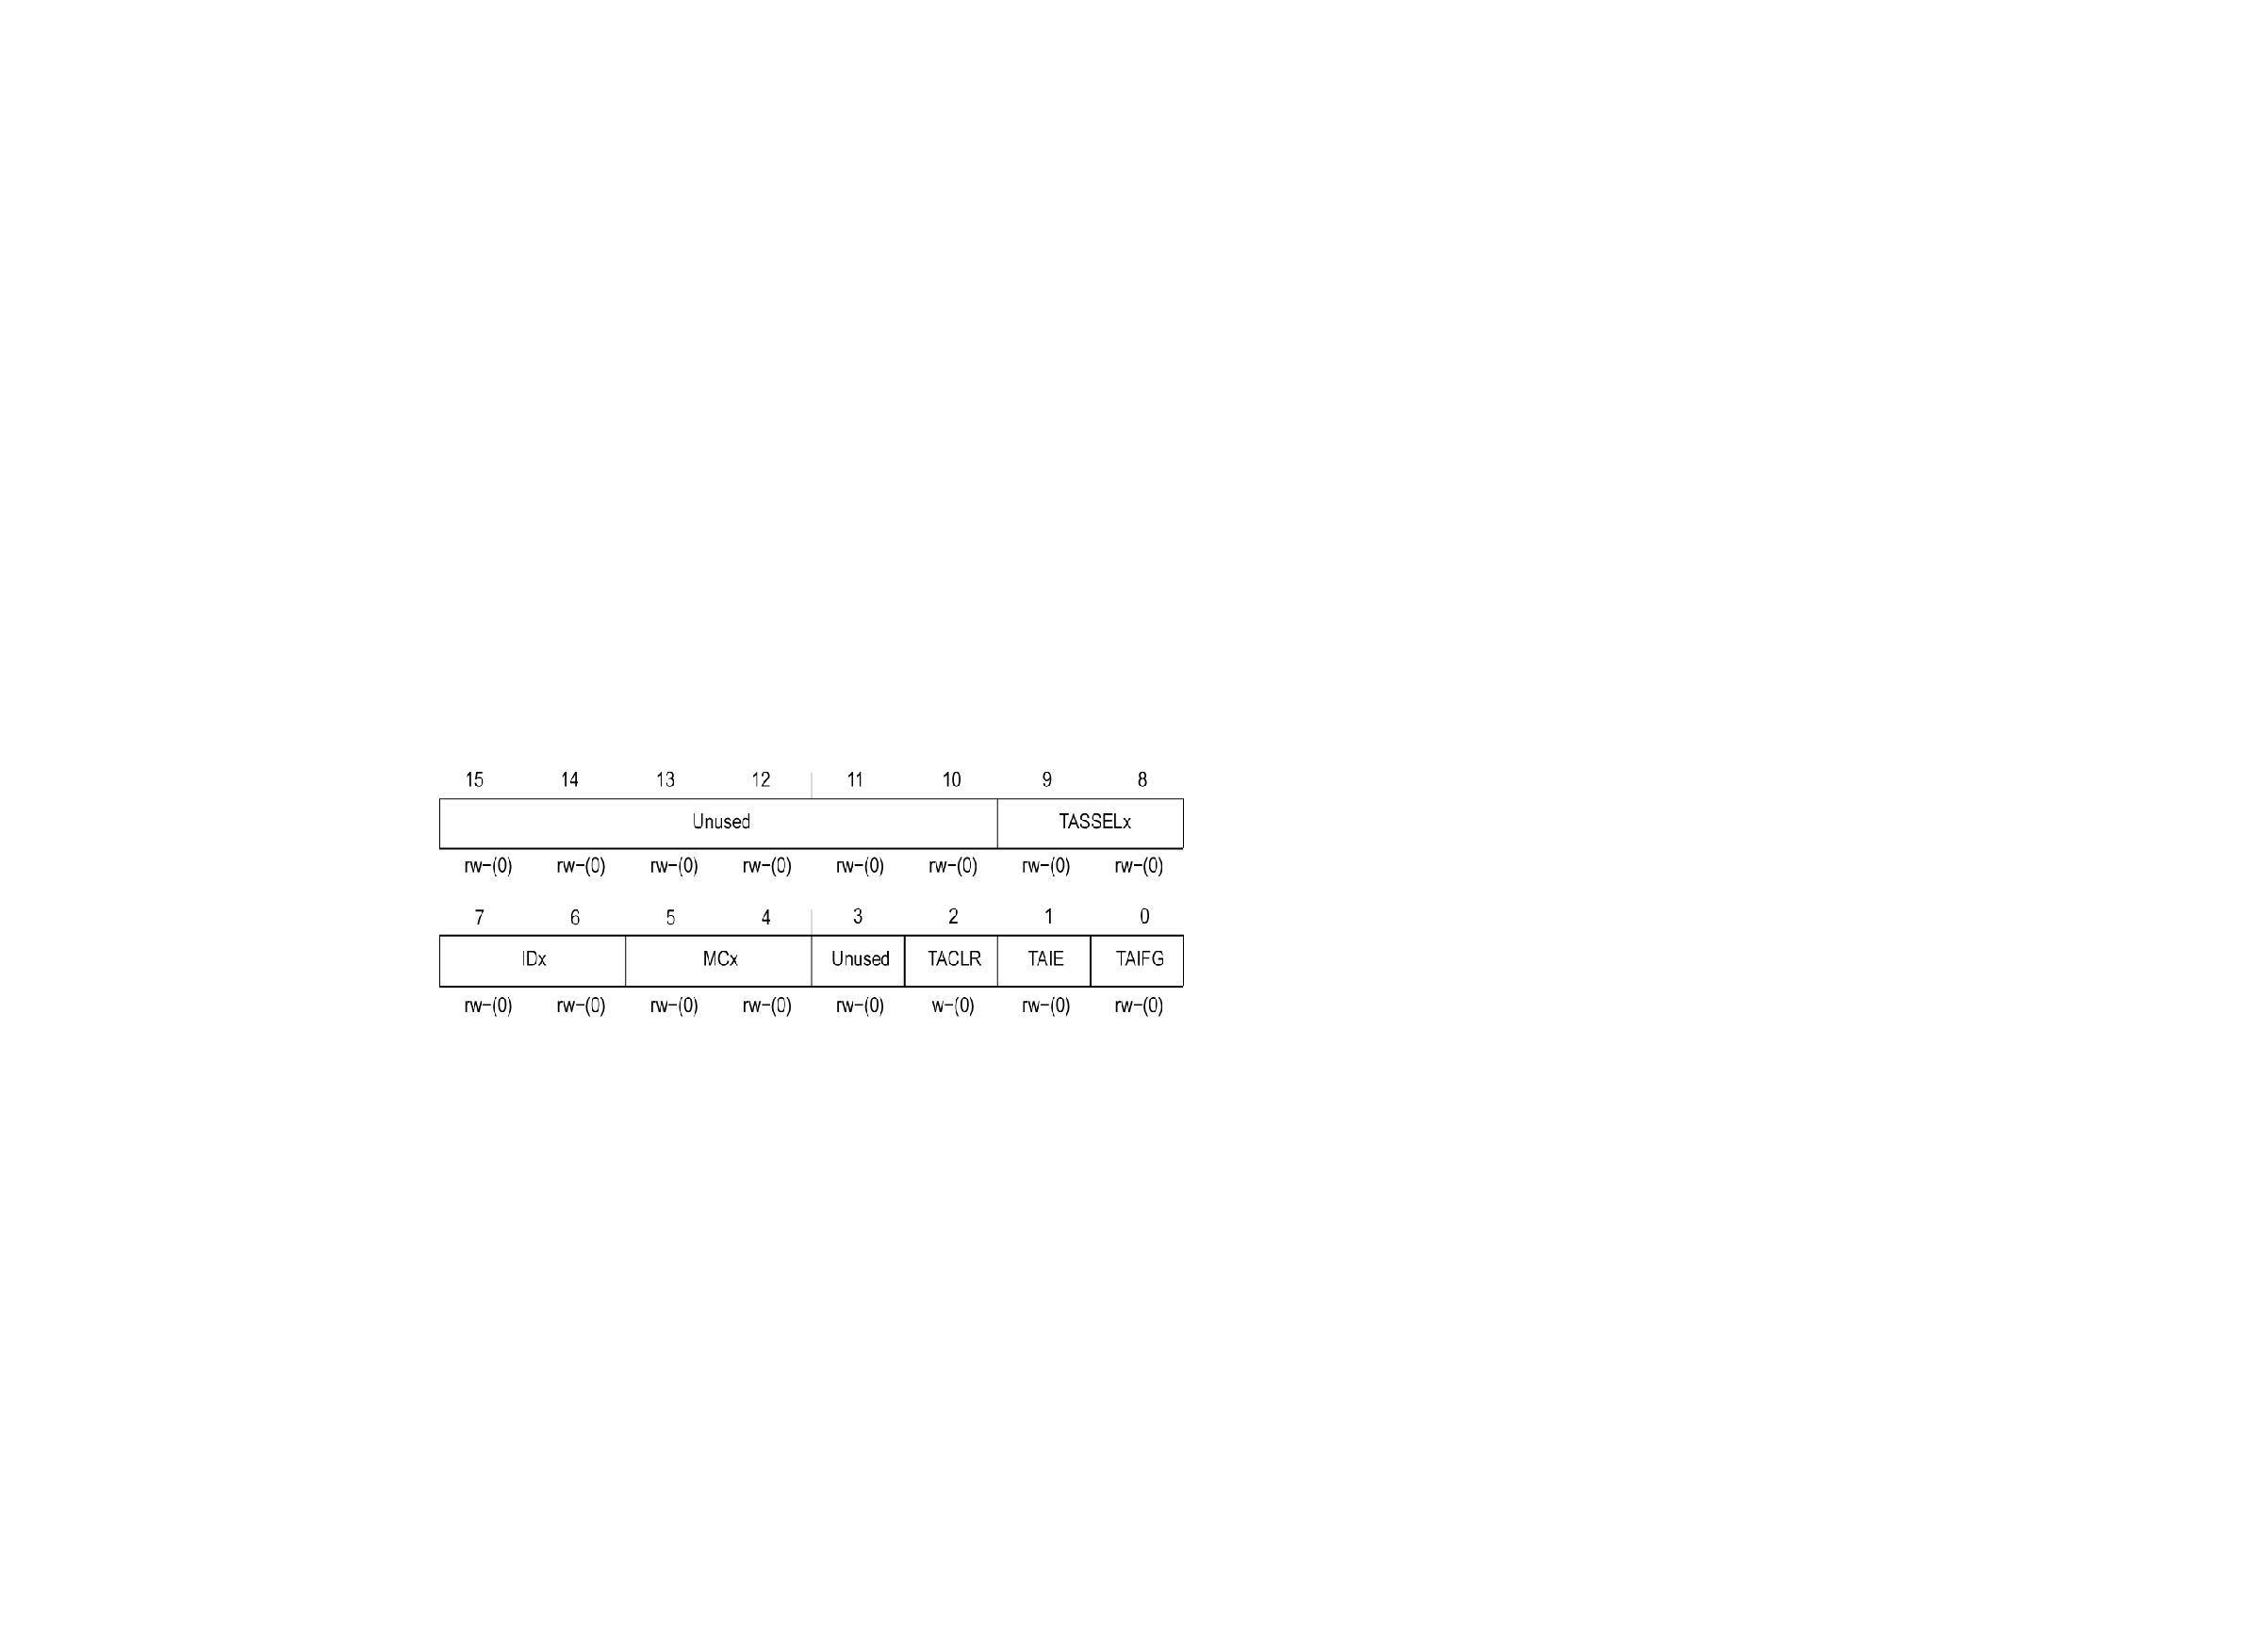
\includegraphics[angle=0, width=13cm]{./Figures/Chap5_Timer/TAxCTL.pdf}
  \rule{35em}{0.5pt}
  \caption[TAxCTL]{Registre TAxCTL}
  \label{fig:TAxCTL}
\end{figure}

\begin{table}[h]
\centering 
\begin{tabular}{l l l l}
\hline\hline
Champ & & Valeur & Description \\ %[0.5ex]
\hline
TASSEL & & & Sélection de l'horloge d'incrémentation  \\
& & 00 & TAxCLK  \\
& & 01 & ACLK  \\
& & 10 & SMCLK  \\
& & 11 & INCLK  \\
\hline
ID & & & Prédivision de l'horloge d'incrémentation  \\
& & 00 & /1  \\
& & 01 & /2  \\
& & 10 & /4  \\
& & 11 & /8  \\
\hline
MC & & & Mode de comptage  \\
& & 00 & Stop. Le timer est arrêté  \\
& & 01 & Mode Up. Le timer compte jusqu'à TAxCCR0  \\
& & 10 & Mode continu. Le timer compte jusqu'à 0xFFFF  \\
& & 11 & Mode Up/Down. Le timer compte jusqu'à TAxCCR0 puis décompte jusqu'à 0  \\
\hline
TACLR & & & Met TAxR à 0. TACLR revient automatiquement à 0 \\
\hline
TAIE & & & Autorisation des requêtes d'interruptions de TAIFG \\
& & 0 & Interruptions non autorisées \\
& & 1 & Interruptions autorisées \\
\hline
TAIFG & & & Indicateur d'interruption \\
& & 0 & Aucune interruption n'est en attente \\
& & 1 & Une interruption est en attente de traitement \\
\hline
\end{tabular}
\caption{Description des champs du registre TAxCTL}
\label{table:TAxCTL}
\end{table}

\begin{minipage}{14cm}{
\subsubsection*{Exemple de configuration}
Les instructions ci-dessous configurent le timer A0 en mode comptage de 0 (inclus) jusqu'à 8191 (inclus), soit 8192 cycles, avec l'horloge SMCLK prédivisée par 8.

\lstset{style=customc}
\begin{lstlisting}
#define TASSEL__SMCLK	(2*0x100u)  /* Timer A clock source select: 2 - SMCLK */
#define ID__8         (3*0x40u)   /* Timer A input divider: 3 - /8 */
#define MC__UP        (1*0x10u)   /* Timer A mode control: 1 - Up to CCR0 */

TA0CCR0 = 8191;
TA0CTL  = TASSEL__SMCLK | MC__UP | ID__8;
\end{lstlisting}
}
\end{minipage}

\subsection{Blocs de capture/comparaison}
Pour enrichir encore les possibilités offertes par le timer A, celui-ci dispose de plusieurs blocs de "capture/comparaison". Selon le type de microcontrôleur, le timer A dispose de 3, 5 ou 7 de ces blocs.
La figure \ref{fig:TimerAstruct} illustre plus en détail la structure du timer A, en mettant en évidence uniquement les registres et les signaux de sortie du timer. Comme dit précédemment, il peut y avoir 3, 5 ou 7 blocs de "capture/comparaison". Sur la figure, n vaut donc 2, 4 ou 6; x est le numéro du timer.

\begin{figure}[H]
  \centering
  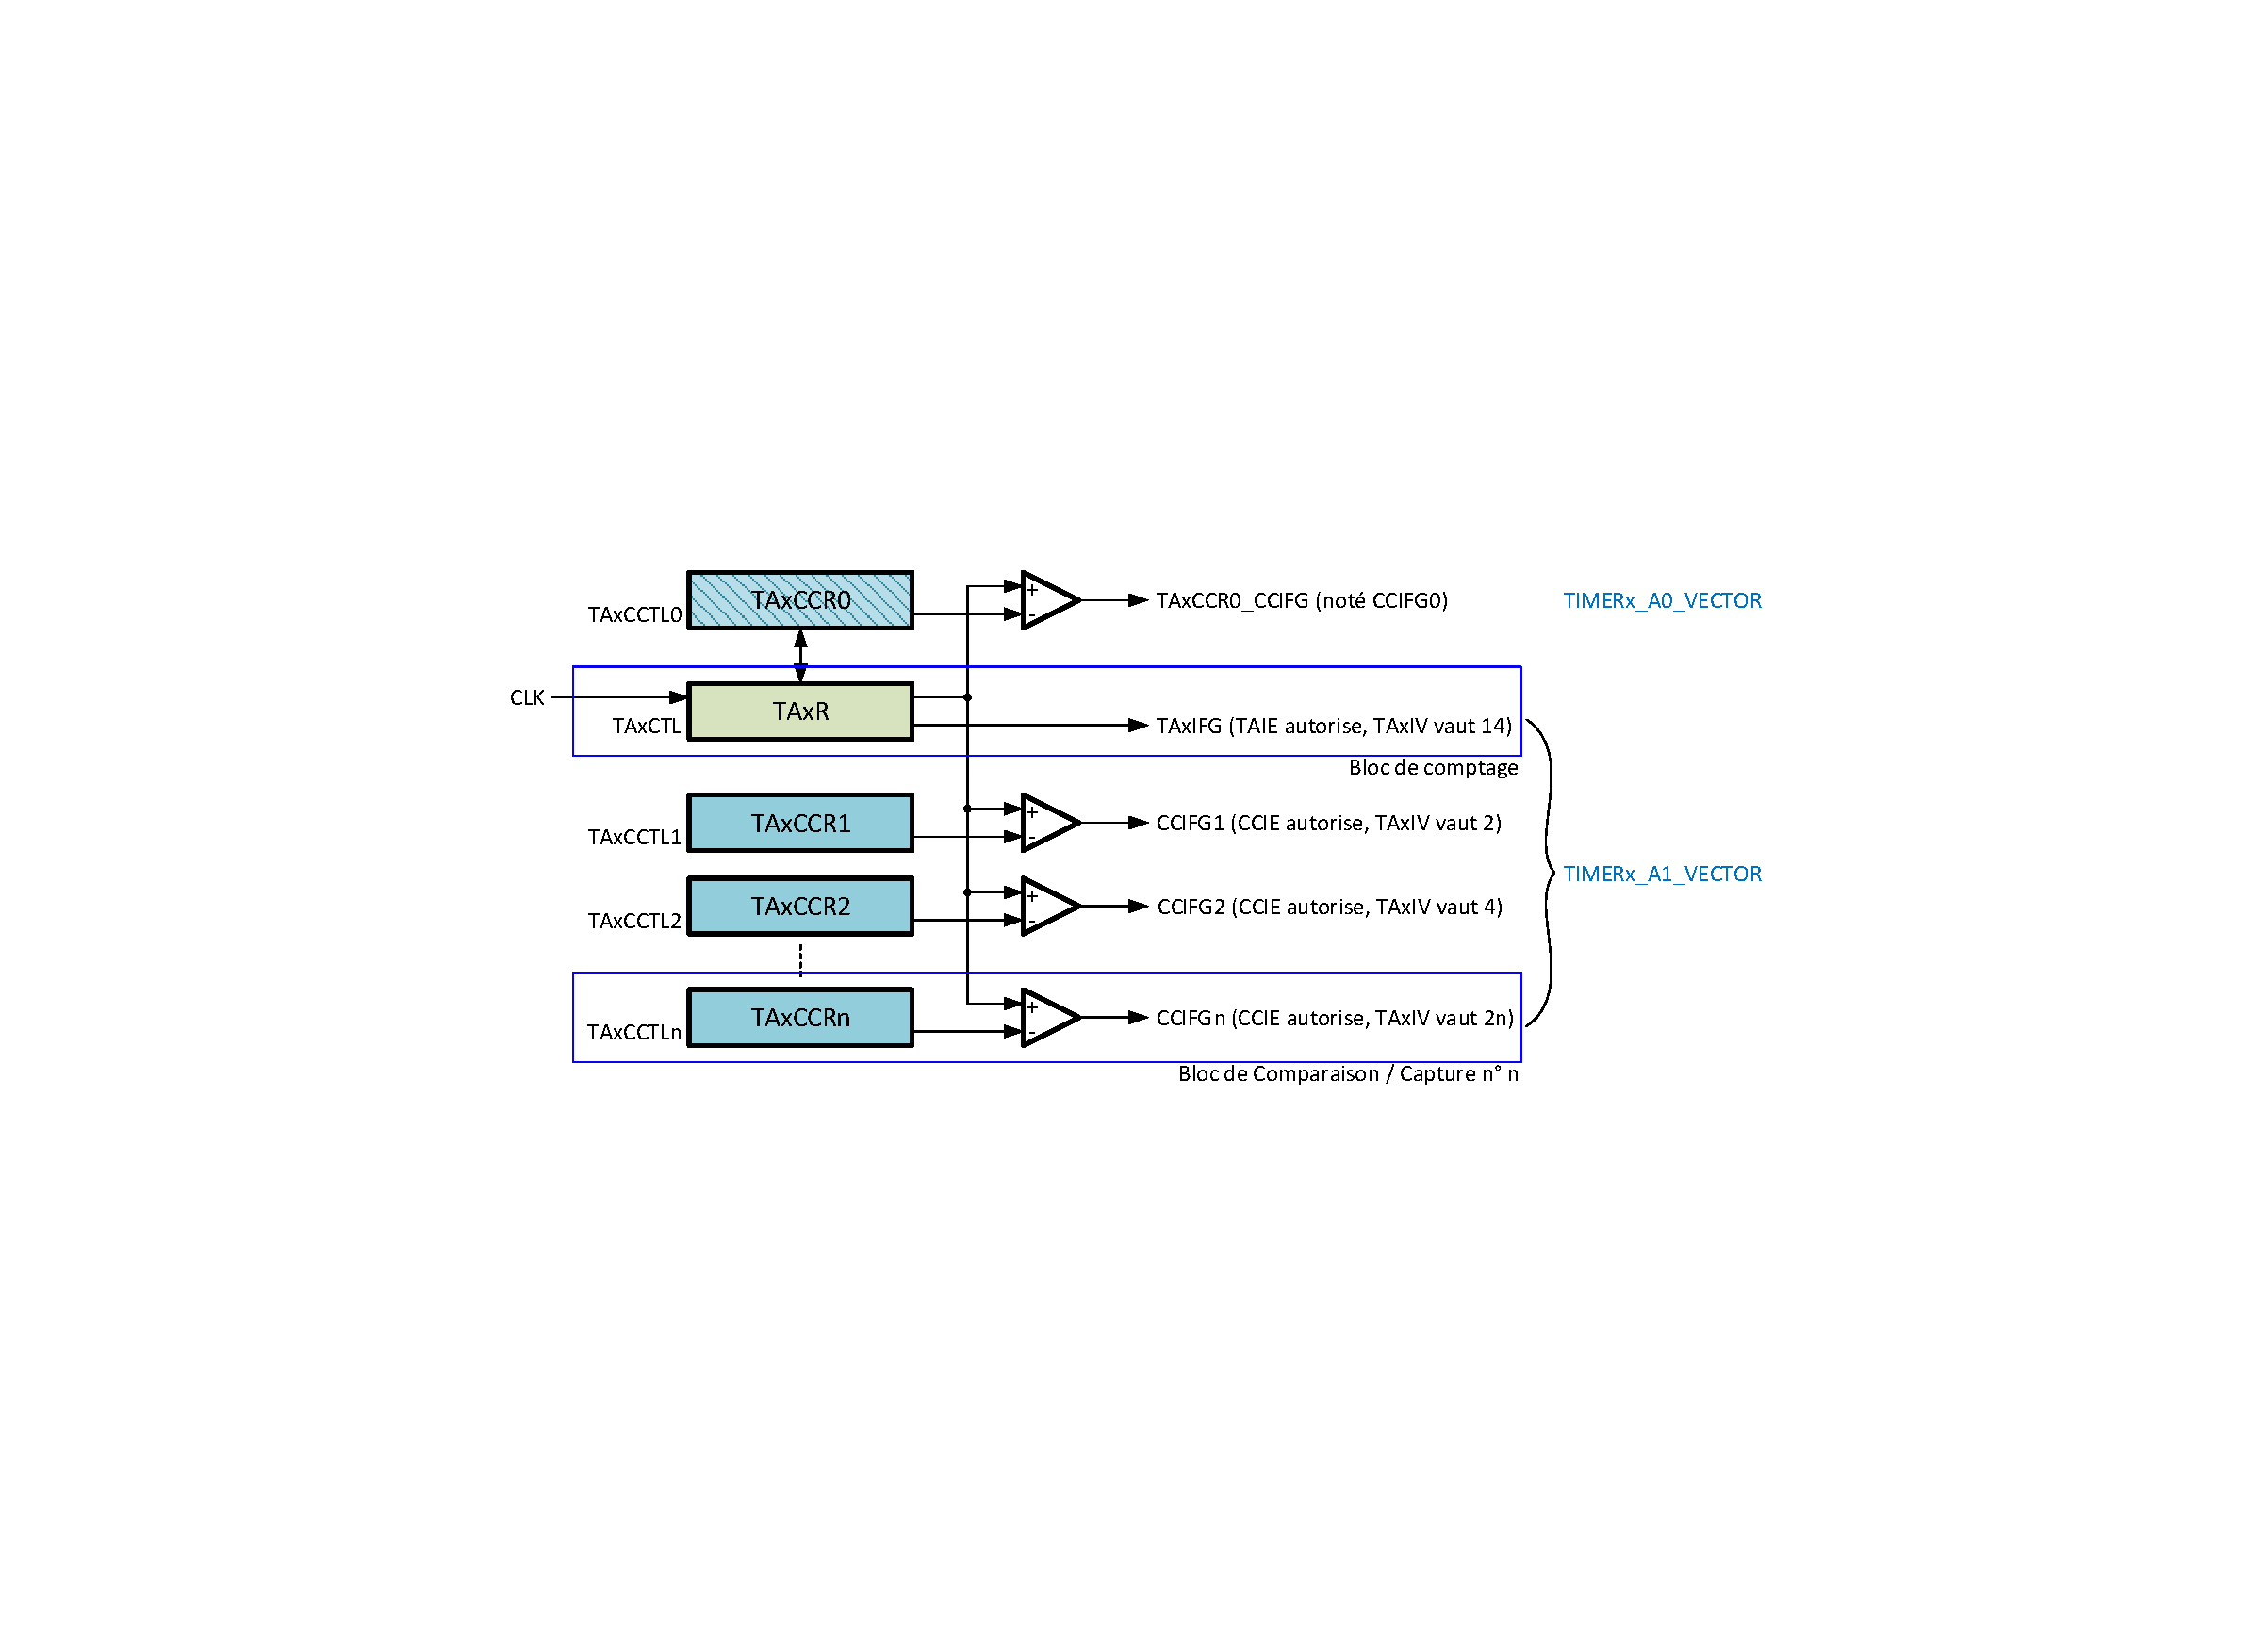
\includegraphics[angle=0, width=15cm]{./Figures/Chap5_Timer/Timer_blocs_3.pdf}
  \rule{35em}{0.5pt}
  \caption[Structure TimerA]{Organisation structurelle du timer A}
  \label{fig:TimerAstruct}
\end{figure}

Le timer est ainsi organisé en tranches, chacune capable de générer ses signaux propres. Dans la figure \ref{fig:TimerAstruct}, chaque rectangle représente un «registre de donnée», c'est à dire un registre qui contient une information représentant une grandeur.
A gauche de chaque «registre de donnée» est noté le nom de son registre de contrôle. Par exemple, à gauche du registre TAxR on retrouve le nom de son registre de contrôle : TAxCTL (TAx ConTroL). Tous ces registres sont sur 16 bits.
Grâce à leur module de sortie, les circuits de capture/comparaison peuvent aussi générer automatiquement des signaux particuliers sur une patte du microcontrôleur. Ces fonctionnalités n'apparaissent pas sur la figure \ref{fig:TimerAstruct}.

\subsection{Contrôle du bloc de capture/comparaison n°0}
Ce bloc fonctionnel est en étroite interaction avec le registre de comptage TAxR, puisqu'il peut (selon la valeur du champ MC) définir la borne supérieure du comptage.

TAxCCR0 : registre de capture/comparaison n° 0 pour le Timer A (n° x). Comme TAxR, TAxCCR0 est un « registre de donnée »; leurs valeurs peuvent être comparées (mode comparaison) ou le contenu de TAxR peut être copié dans TAxCCR0 (mode capture).
Lors de ces deux événements (égalité des deux registres ou transfert de TAxR dans TAxCCR0), une requête d'interruption est émise; c'est le signal appelé TAxCCR0\_CCIFG, que nous nommerons CCIFG0.
Ce circuit de capture/compare, centré autour du registre TAxCCR0, est contrôlé par le registre de contrôle TAxCCTL0.

TAxCCTL0 : registre de contrôle du circuit de capture/compare n° 0 pour le Timer A (n° x). Il permet de spécifier comment TAxCCR0 se comporte. Il est composé de 6 champs, pour:
\begin{itemize}[label=\textbullet,font=\small]
\item sélectionner la fonction Capture ou Comparaison (CAP)
\item sélectionner le mode de capture (sur flanc montant, descendant, etc...) (CM)
\item sélectionner le signal de capture (CCIS)
\item synchroniser ou non du signal de capture avec l'horloge de comptage (SCS)
\item sélectionner le mode de sortie (OUTMOD)
\item autoriser ou non les interruptions émises par le bloc de capture comparaison n° 0 (CCIE)
\end{itemize}

D'autres champs contiennent différents signaux tels que le flag de l'interruption issue du bloc (CCIFG0).
\\
La figure \ref{fig:TimerCCR} illustre en détail un bloc de capture/comparaison (n° y). On y voit les différents sous blocs et leurs champs de contrôle, tous éléments du registre de contrôle TAxCCTLy.

\begin{figure}[h]
  \centering
  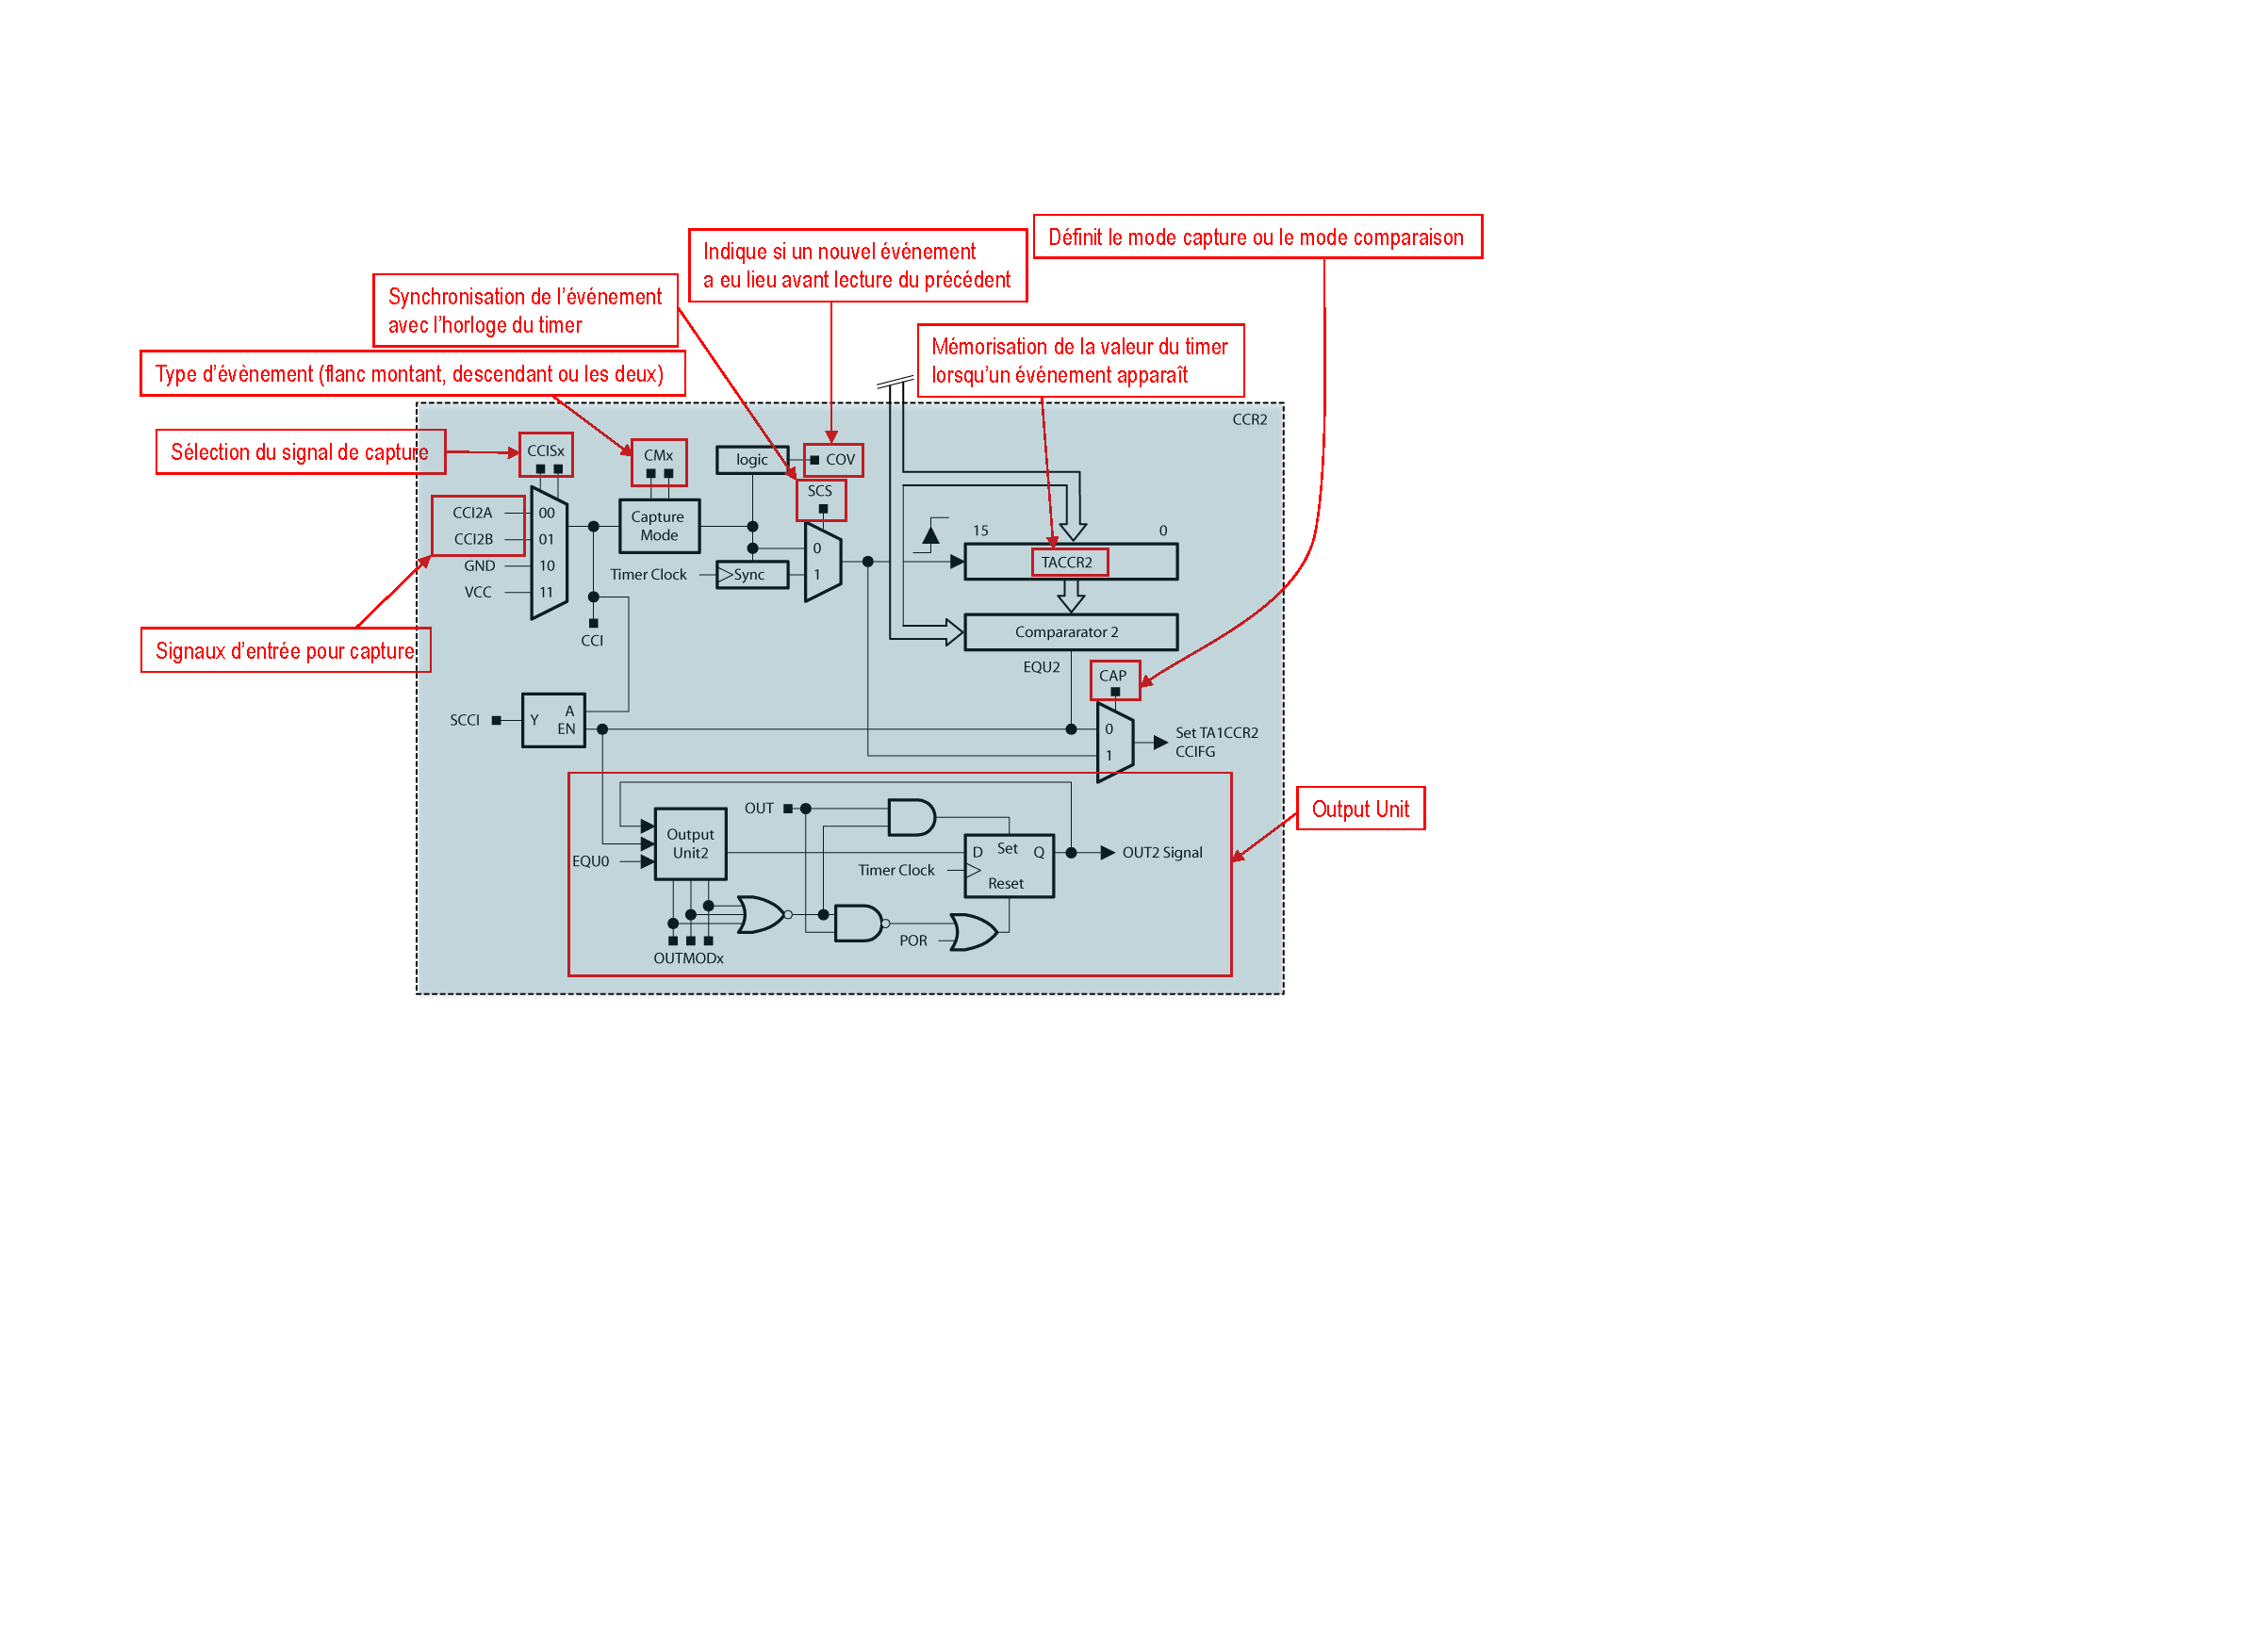
\includegraphics[angle=0, width=16cm]{./Figures/Chap5_Timer/Timer_Detail_2.pdf}
  \rule{35em}{0.5pt}
  \caption[TimerCCR]{Schéma de détail du bloc de capture/comparaison}
  \label{fig:TimerCCR}
\end{figure}

Le détail du registre de contrôle TAxCCTLy, pour le bloc de capture/comparaison n°y, est donné à la figure \ref{fig:TAxCCTLy} et dans le tableau \ref{table:TAxCCTL}. 

\begin{figure}[H]
  \centering
  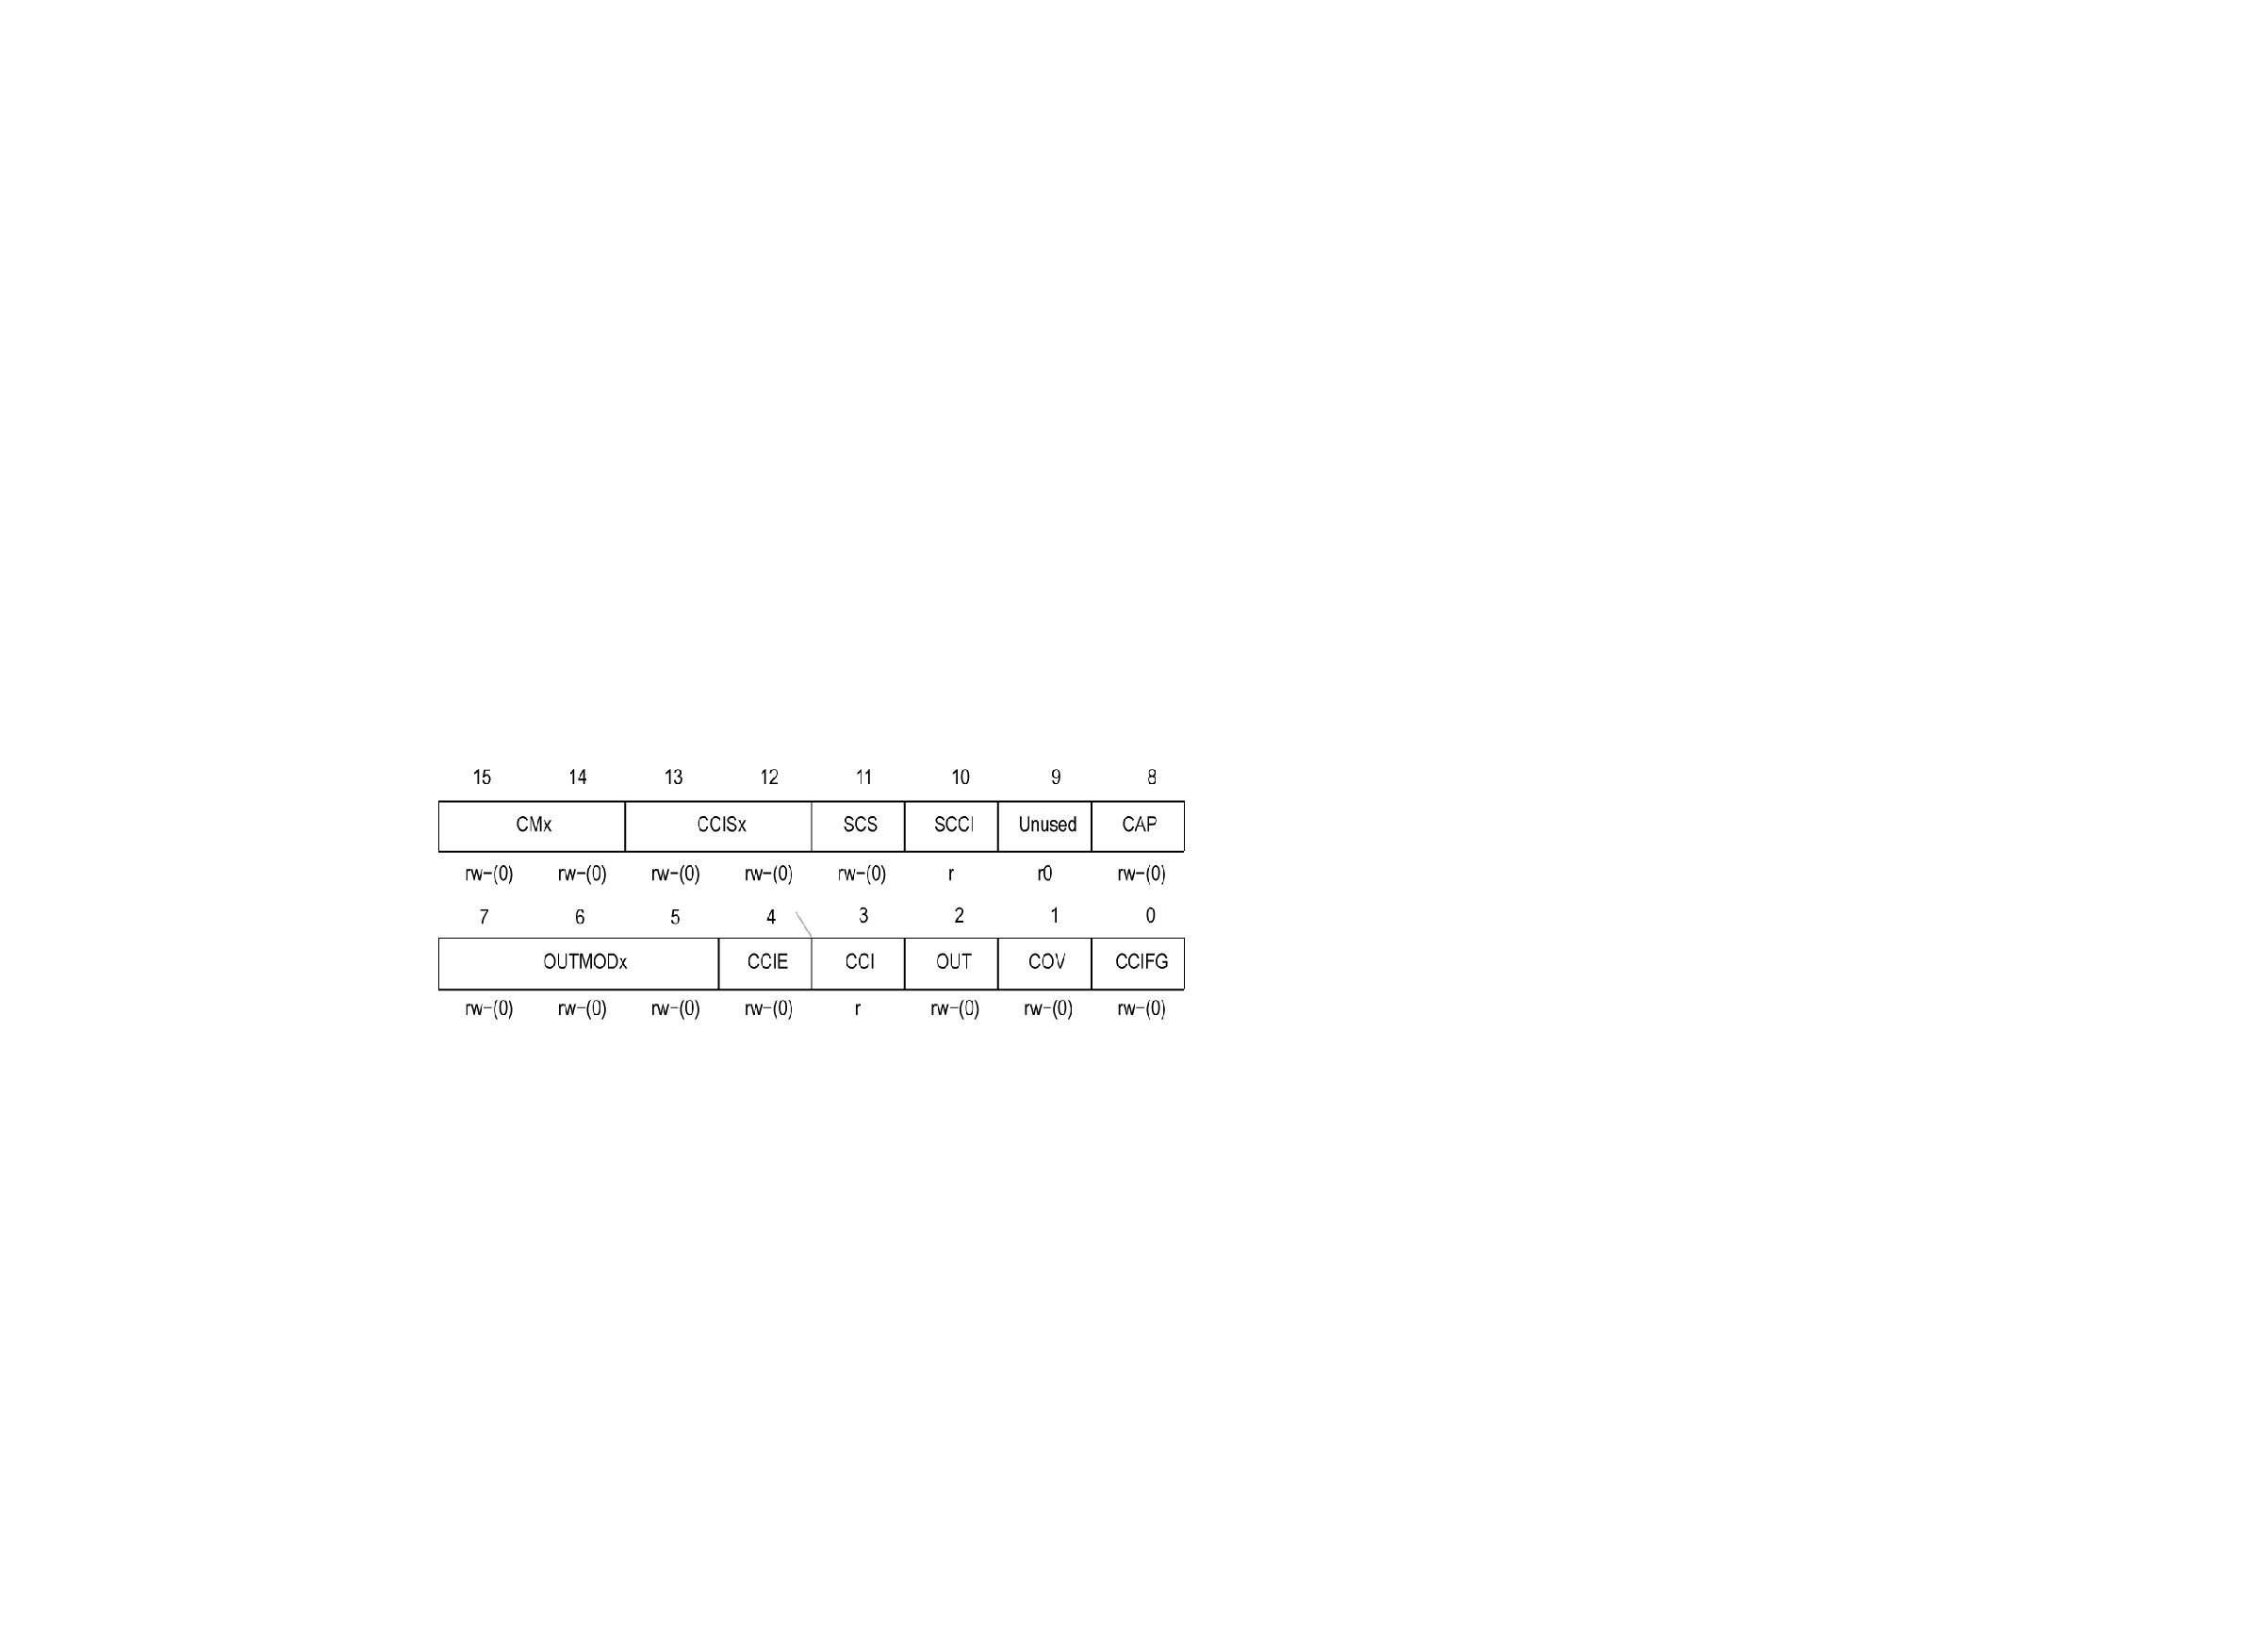
\includegraphics[angle=0, width=13cm]{./Figures/Chap5_Timer/TAxCCTLy.pdf}
  \rule{35em}{0.5pt}
  \caption[TAxCCTLy]{Registre TAxCCTLy}
  \label{fig:TAxCCTLy}
\end{figure}

\begin{table}[H]
\centering 
\begin{tabular}{l l l l}
\hline\hline
Champ & & Valeur & Description \\ %[0.5ex]
\hline
CM & & & Mode de capture  \\
& & 00 & Pas de capture  \\
& & 01 & Capture sur le flanc montant du signal de capture  \\
& & 10 & Capture sur le flanc descendant  \\
& & 11 & Capture sur les deux flancs  \\
\hline
CCIS & & & Sélection du signal de capture  \\
& & 00 & CCIxA  \\
& & 01 & CCIxB  \\
& & 10 & GND  \\
& & 11 & VCC  \\
\hline
SCS & & & Synchronisation du signal de capture  \\
& & 0 & Pas de synchronisation \\
& & 1 & Synchronisation du signal de capture avec le prochain flanc de CLK \\
\hline
SCCI & & & Image du signal de capture après synchronisation \\
\hline
CAP & & & Sélection entre capture et comparaison \\
& & 0 & Mode comparaison \\
& & 1 & Mode capture \\
\hline
OUTMOD & & & Génération du signal de sortie OUT (module de sortie) \\
& & &  voir chapitre \ref{Module de sortie} \\ 
\hline
CCIE & & & Autorisation des requêtes d'interruptions de CCIFG \\
& & 0 & Interruptions non autorisées \\
& & 1 & Interruptions autorisées \\
\hline
\end{tabular}
\caption{Description des champs du registre TAxCCTL}
\label{table:TAxCCTL}
\end{table}

\subsubsection*{Exemple de configuration}
Les instructions ci-dessous reprennent la configuration vue au chapitre 5.3.2, en autorisant de plus le bloc de capture/comparaison du timer A0 à émettre des requêtes d'interruptions par son signal CCIFG0.

\lstset{style=customc}
\begin{lstlisting}
#define TASSEL__SMCLK (2*0x100u) /* Timer clock source select: 2 - SMCLK */
#define ID__8         (3*0x40u) /* Timer input divider: 3 - /8 */
#define MC__UP        (1*0x10u) /* Timer mode control: 1 - Up to CCR0 */
#define CCIE          (1*0x10u) /* Capture/compare interrupt enable */

TA0CCR0 = 8191;
TA0CTL  = TASSEL__SMCLK | MC__UP | ID__8;
TA0CCTL0  = CCIE;
\end{lstlisting}

\subsection{Contrôle des blocs de capture/comparaison n°1,2,3...}
Ces circuits sont des copies conformes du circuit de capture/comparaison n° 0. La seule différence est que leur registre central (TAxCCRy) n'a pas d'influence sur la borne supérieure de TAxR. Ils interagissent toutefois avec TAxR en mode capture.
Pour le circuit n° y, le registre de donnée est nommé TAxCCRy, le registre de contrôle est TAxCCTLy.
Bien entendu, dans le registre de contrôle TAxCCTLy, les champs portent les même noms (CAP, CM, CCIS, SCS, etc...).

\subsection{Différence entre Capture et Comparaison}
La figure \ref{fig:CapvsComp} illustre le comportement du registre TAxR dans le mode 1 (continuous).

\begin{figure}[h]
  \centering
  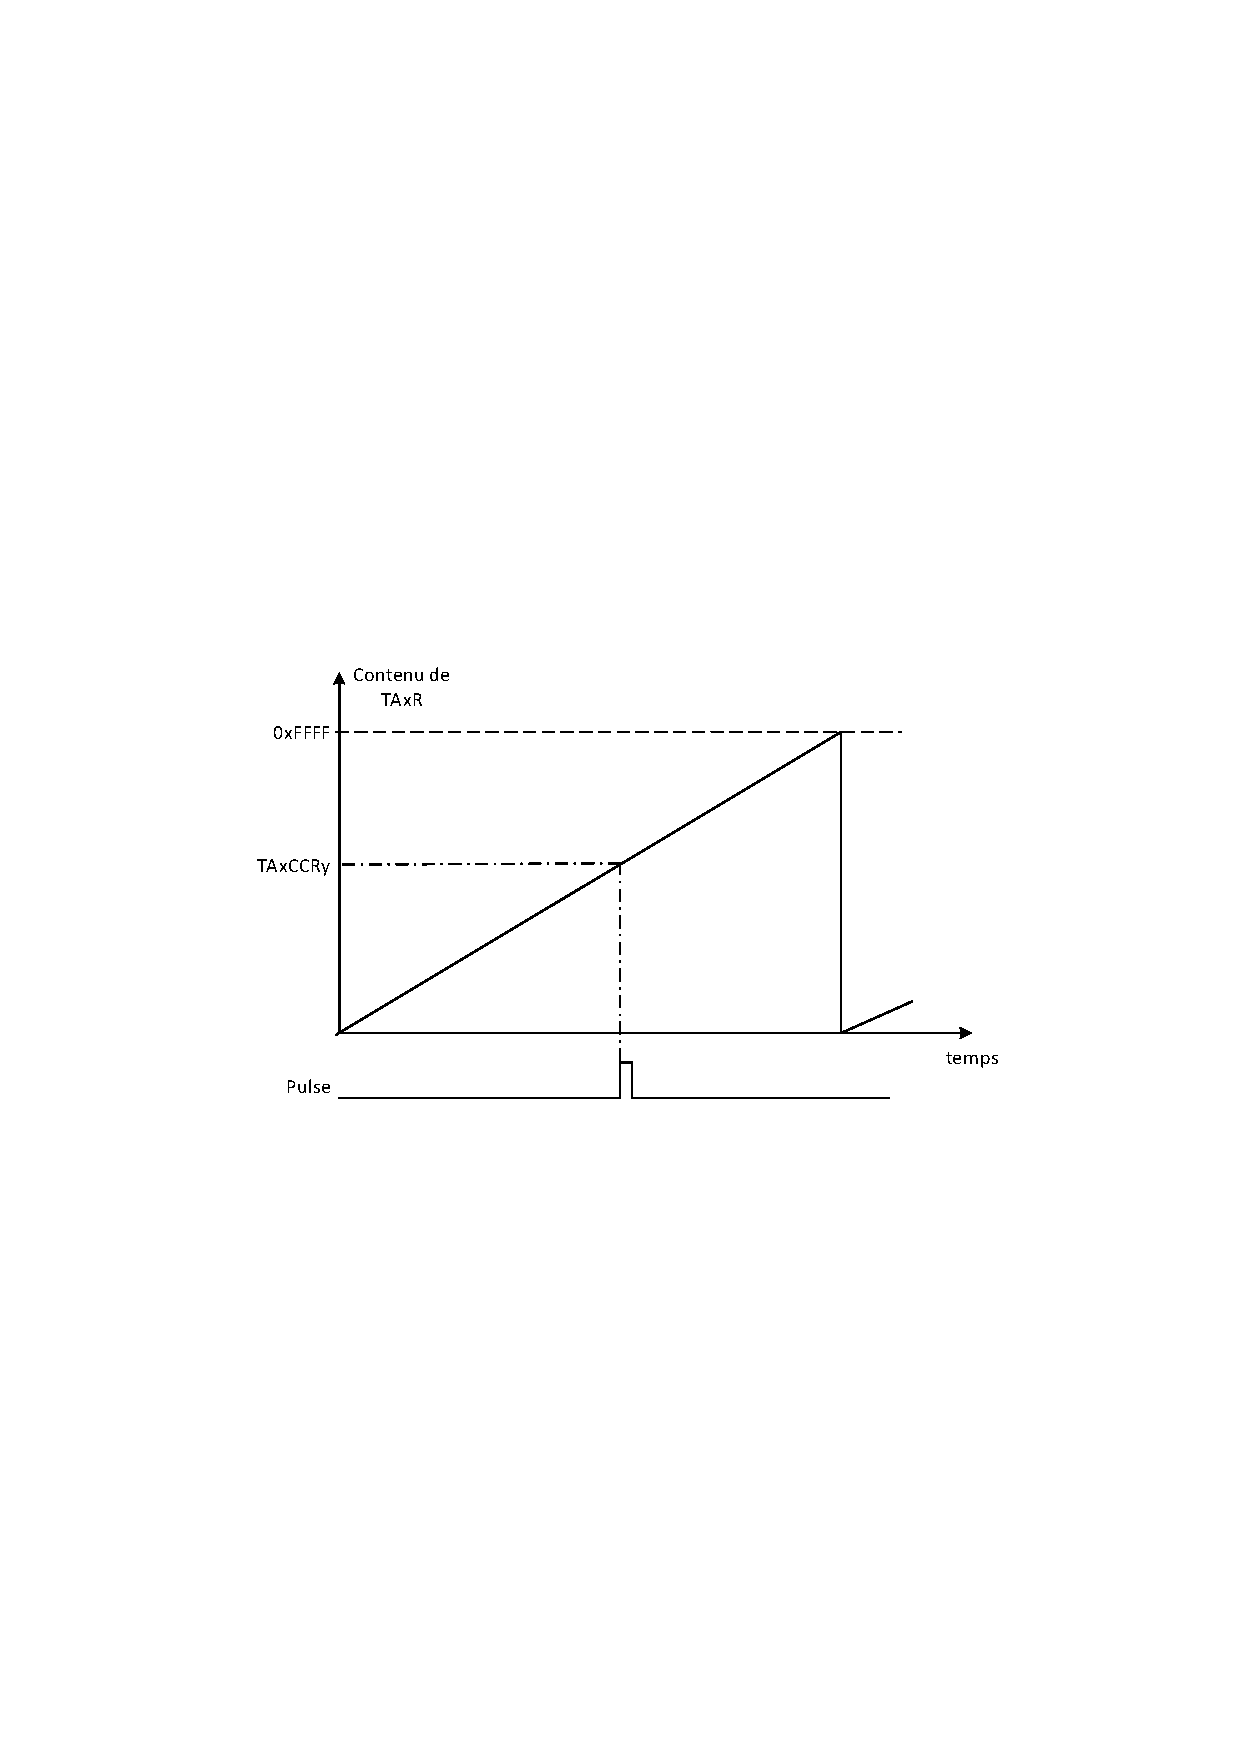
\includegraphics[angle=0, width=14cm]{./Figures/Chap5_Timer/Timer_CC.pdf}
  \rule{35em}{0.5pt}
  \caption[CapvsComp]{Comparaison : TAxR est l'entrée / Capture : Pulse est l'entrée}
  \label{fig:CapvsComp}
\end{figure}

Une fois le processus de comptage lancé, TAxR évolue en dent de scie, comme illustré. Le circuit de capture/comparaison utilise ce signal pour son opération.

En mode « comparaison », le contenu du registre TAxCCRy est une entrée. Dès que TAxR atteint TAxCCRy, le signal noté « Pulse » est généré, qui peut déclencher l'exécution d'une routine de service d'interruption. En mode « comparaison », le signal appelé « Pulse » dans la figure \ref{fig:CapvsComp} est en fait CCIFG.

En mode « capture », le contenu du registre TAxCCRy est une sortie. Un signal « Pulse » doit être fourni, qui déclenche la copie de TAxR dans TAxCCRy au moment où la pulse apparaît. En fait, c'est le flanc actif de la pulse qui déclenche le processus de capture, qui peut donc se produire sur le flanc montant, descendant ou les deux, du signal « pulse ». Typiquement, le signal « pulse » est une entrée du microcontrôleur. Au moment où la capture est exécutée, une requête d'interruption peut être émise.

\subsection{Interruptions du timer A}
Un timer A contenant n bloc de capture/comparaison peut générer $n+1$ requêtes d'interruptions. Toutefois, seuls deux vecteurs d'interruption sont définis. 
Revenant à la figure \ref{fig:TimerAstruct}, on voit que le signal CCIFG0 issu du bloc de capture/comparaison n°0 est associé à lui tout seul à un des vecteurs (TIMERx\_A0\_VECTOR). Tous les autres signaux d'interruption (TAxIFG, CCIFG1, CCIFG2, ...) sont associés à l'autre vecteur (TIMERx\_A1\_VECTOR).

Si une interruption provient d'un des signaux TAIFG, CCIFG1 ou CCIFG2, il est donc nécessaire de tester lequel de ces signaux est effectivement responsable de la requête. L'information y relative est disponible dans registre particulier TAIV, appelé abusivement "vecteur d'interruption". Il est ainsi possible de déterminer rapidement la source de l'interruption, en testant la valeur de TAIV au moyen d'une instruction \textit{SWITCH...CASE}.

La description du registre TAIV est donnée à la table \ref{table:TAIV} :
\begin{table}[htb]
\centering 
\begin{tabular}{l l l}
\hline\hline
Champ & Valeur & Source de l'interruption \\ %[0.5ex]
\hline                  % inserts single horizontal line
TAIV & 0x00 & pas d'interruption en attente  \\	% inserting body of the table
& 0x02 & CCIFG1  \\
& 0x04 & CCIFG2  \\
& 0x06 & CCIFG3  \\
& 0x08 & CCIFG4  \\
& 0x0A & CCIFG5  \\
& 0x0C & CCIFG6  \\
& 0x0E & TAIFG  \\ [1ex]      % [1ex] adds vertical space
\hline
\end{tabular}
\caption{Description du registre TAIV}
\label{table:TAIV}
\end{table}

\begin{minipage}{16cm}{
\subsubsection*{Exemple de programme avec interruption}
Le code ci-dessous configure le timer A en mode continu (jusqu'à 0xFFFF). Le signal TAIFG s'active lors du passage de TAxR à 0, et émet une requête d'interruption. Dans la routine d'interruption, la patte n°1 du port P5 change d'état.

\lstset{style=customc}
\begin{lstlisting}
#include <msp430.h>

#define MC__CONTINUOUS  (2*0x10u)  /* Timer A mode control: 2 - Continuous up */

void main(void)
{
  WDTCTL = WDTPW + WDTHOLD;              // Stop watchdog timer
  P5DIR |= 0x02;
  TACTL = TASSEL__SMCLK + MC__CONTINUOUS + TAIE;
  
  _enable_interrupts();
  
  while(1);
}

// Timer_A1 Interrupt Vector (TAIV) handler
#pragma vector=TIMER0_A1_VECTOR
__interrupt void timer_a0_ccr1_isr(void)
{
  switch(__event_in_range(TA0IV, TA0IV_TAIFG))
  {
  case TA0IV_NONE:   break;
  case TA0IV_TACCR1: break;
  case TA0IV_TACCR2: break;
  case TA0IV_TACCR3: break;
  case TA0IV_TACCR4: break;
  case TA0IV_TAIFG:
    P5OUT ^= 0x02;
    break;
  default: break;
  }
}
\end{lstlisting}
}
\end{minipage}

\subsection{Module de sortie}
\label{Module de sortie}
Dans chaque bloc de capture/comparaison, le module de sortie est capable de générer plusieurs types de signaux sur sa sortie OUT. Il est possible de connecter ce signal OUT vers une patte du microcontrôleur, en configurant le port correspondant au moyen du registre PxSEL.
Il est nécessaire de consulter la fiche technique du microcontrôleur utilisé pour savoir quelles pattes peuvent être connectées à quels modules de sortie de timer.

La génération du signal OUT est basée sur deux signaux EQU0 et EQUy internes aux circuits de capture/comparaison n° 0 et y:
\begin{itemize}[label=\textbullet,font=\small]
\item EQU0 s'active quand TAxR = TAxCCR0
\item EQUy s'active quand TAxR = TAxCCRy
\end{itemize}
Elle dépend aussi du mode de comptage dans lequel se trouve le bloc de comptage.

Les figures \ref{fig:Outmod_MC1}, \ref{fig:Outmod_MC2} et \ref{fig:Outmod_MC3} montrent l'évoluetion du signal de sortie OUT en fonction du mode de comptage, pour chaque valeur du champ OUTMOD (registre TAxCCTLy).

\begin{figure}[t]
  \centering
  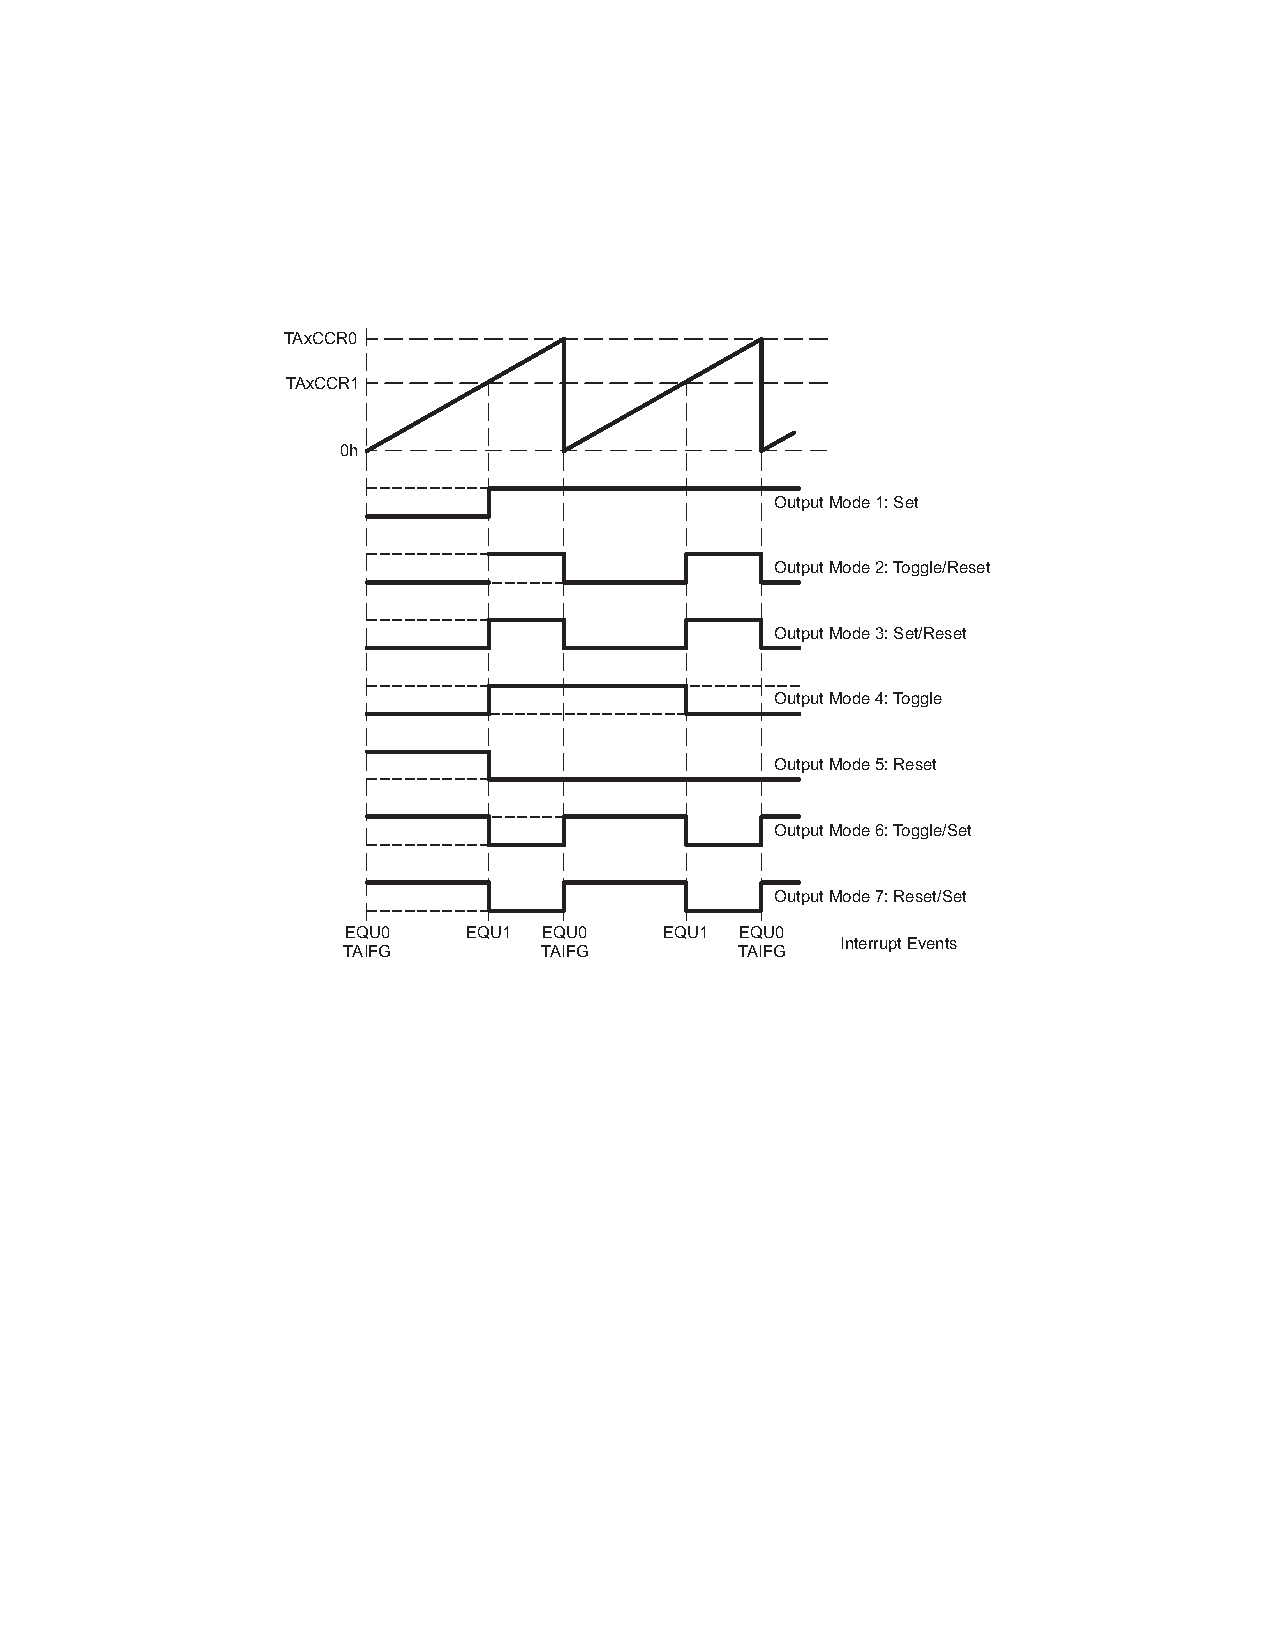
\includegraphics[angle=0, width=14cm]{./Figures/Chap5_Timer/Timer_Out1.pdf}
  \rule{35em}{0.5pt}
  \caption[Outmod_MC1]{Exemple de sortie - TimerA en mode Up (MC = 01)}
  \label{fig:Outmod_MC1}
\end{figure}

\begin{figure}[t]
  \centering
  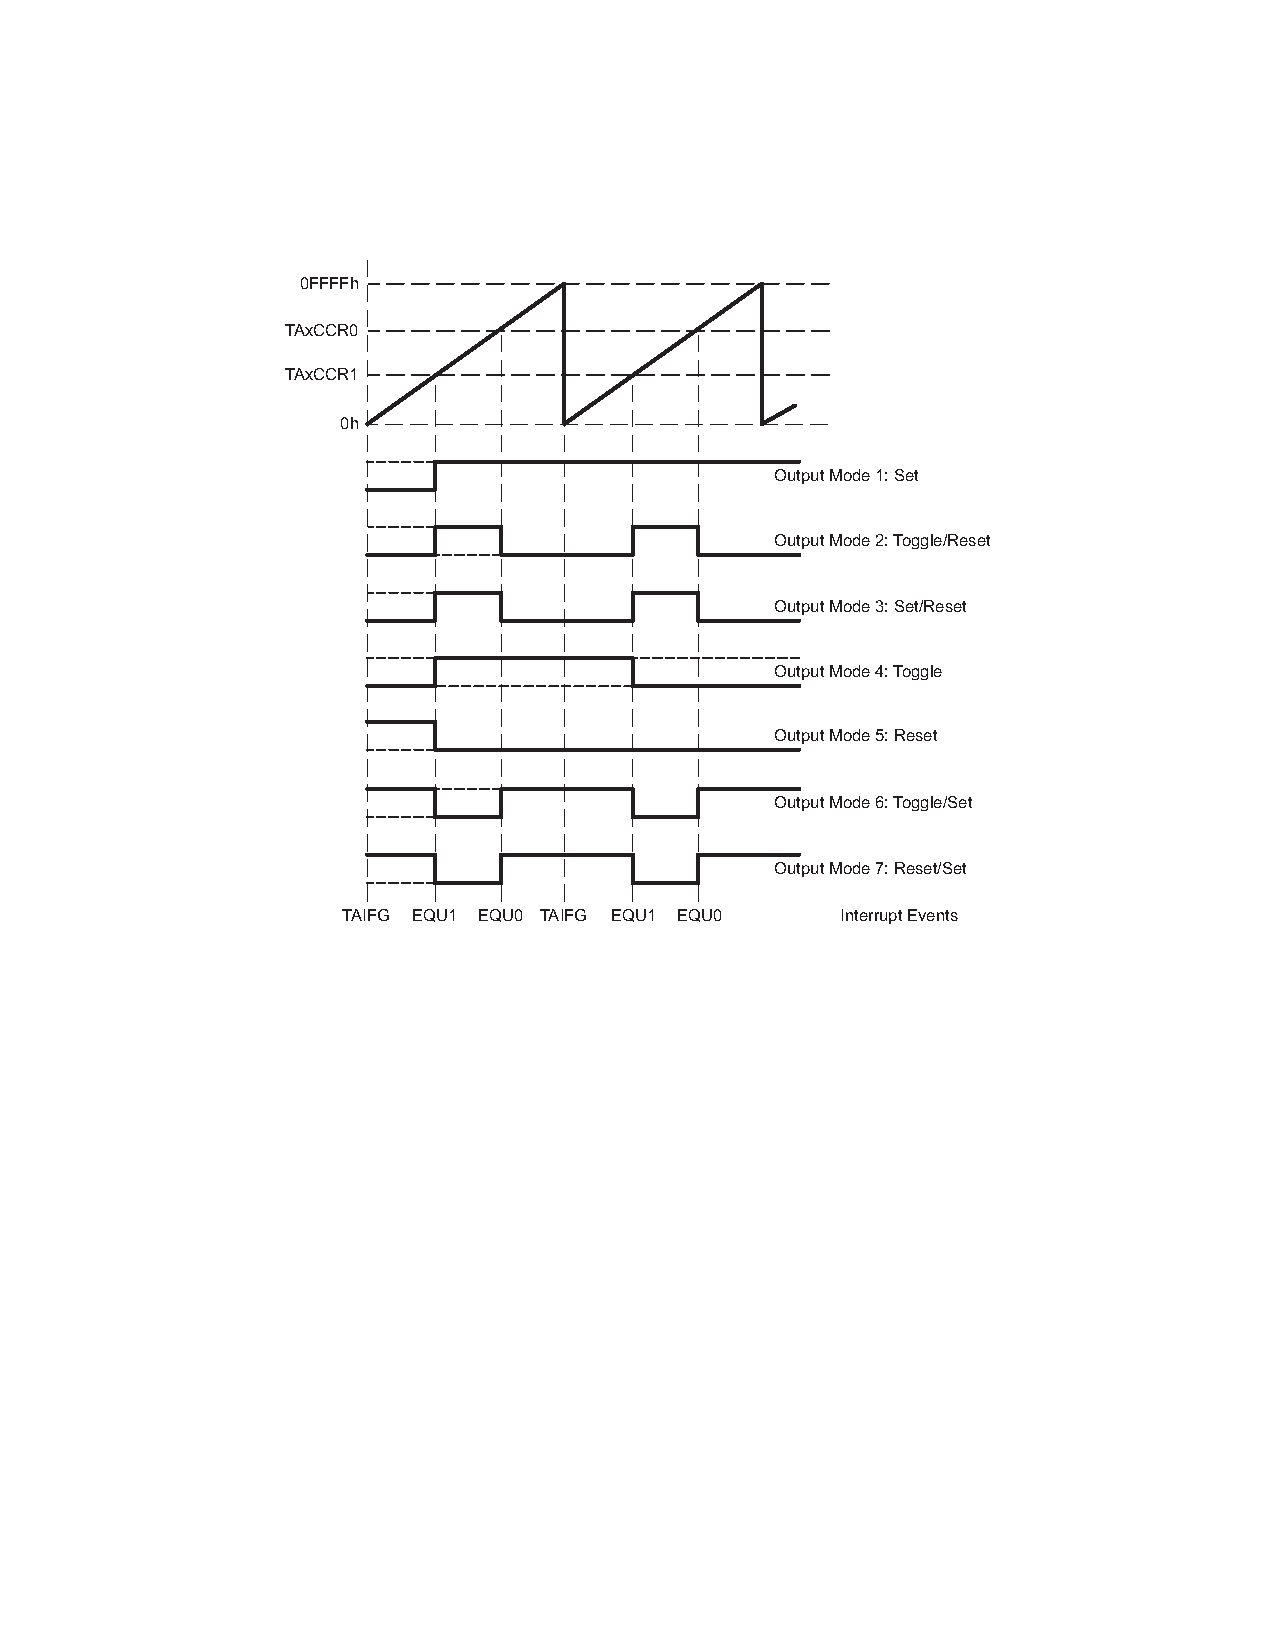
\includegraphics[angle=0, width=14cm]{./Figures/Chap5_Timer/Timer_Out2.pdf}
  \rule{35em}{0.5pt}
  \caption[Outmod_MC2]{Exemple de sortie - TimerA en mode Continu (MC = 10)}
  \label{fig:Outmod_MC2}
\end{figure}

\begin{figure}[t]
  \centering
  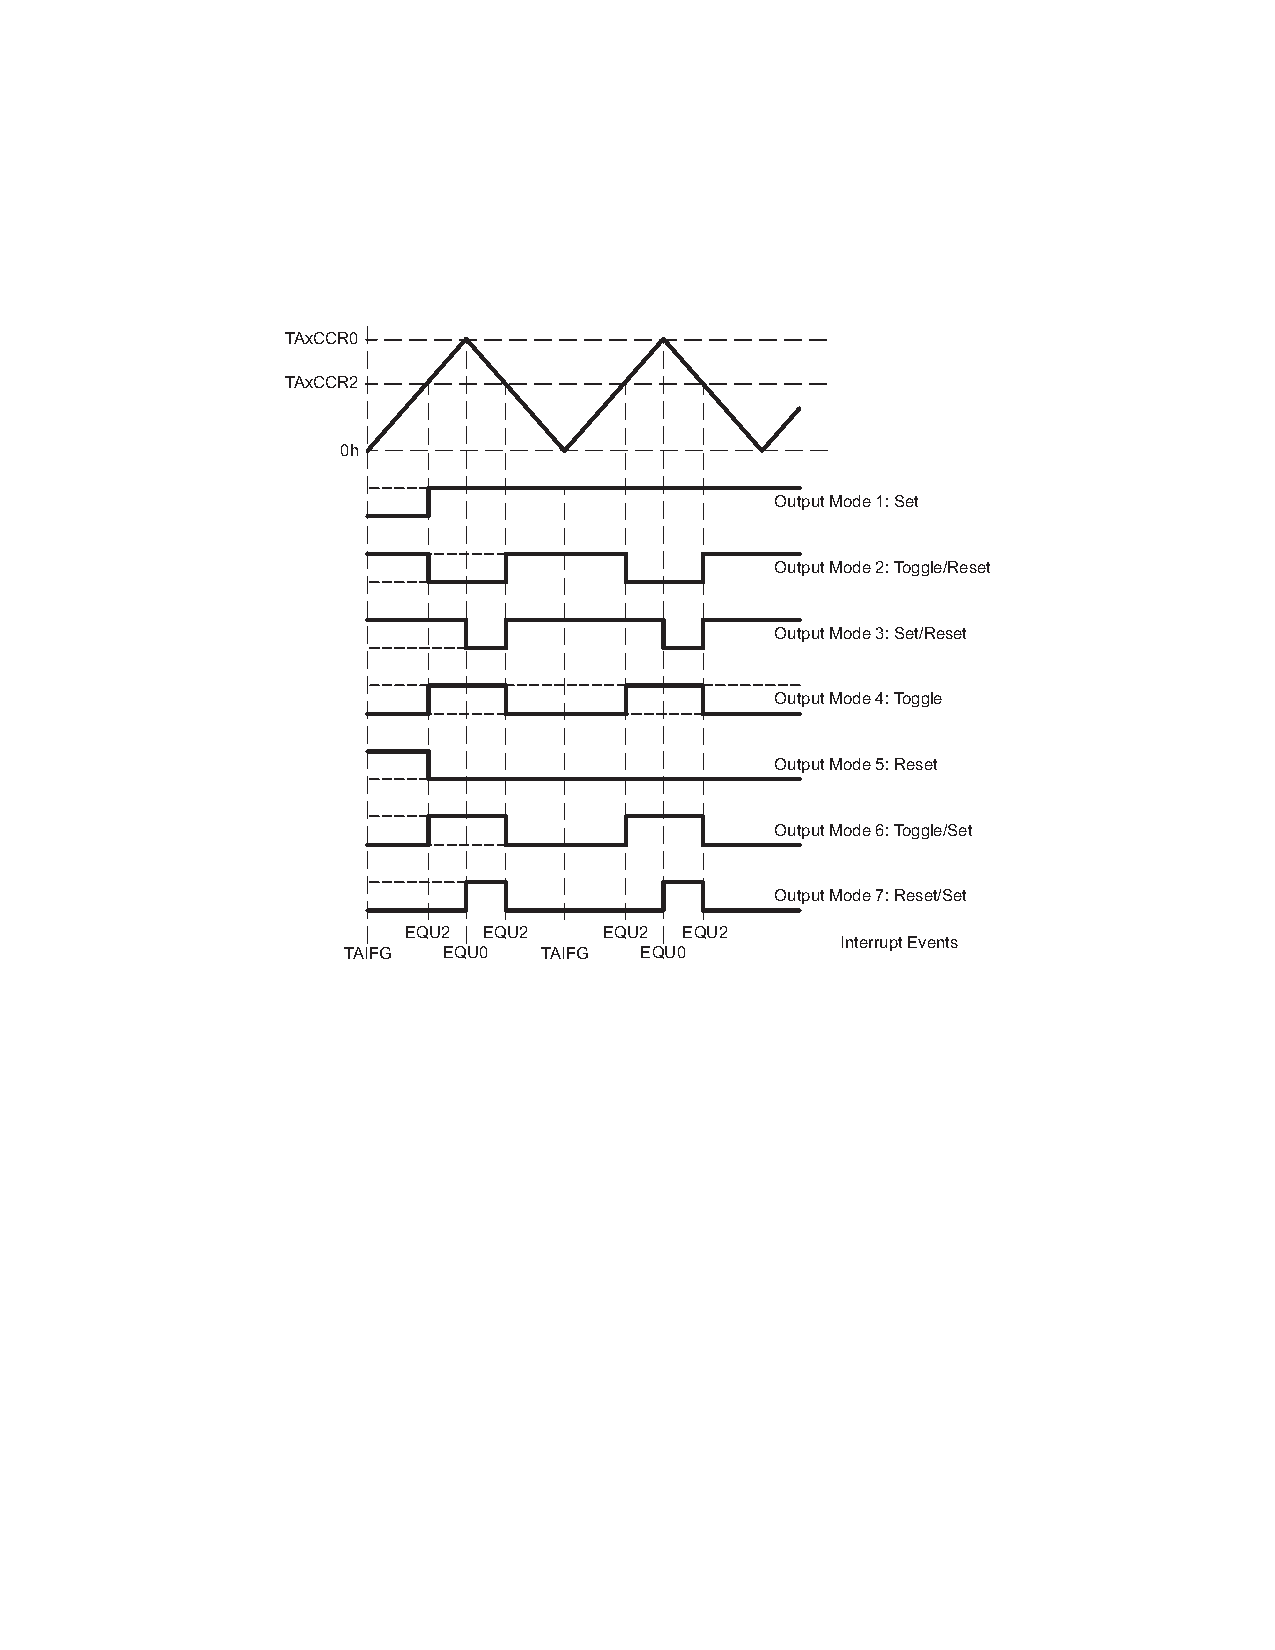
\includegraphics[angle=0, width=14cm]{./Figures/Chap5_Timer/Timer_Out3.pdf}
  \rule{35em}{0.5pt}
  \caption[Outmod_MC3]{Exemple de sortie - TimerA en mode Up/Down (MC = 11)}
  \label{fig:Outmod_MC3}
\end{figure}








